% !TeX root = ../../../main.tex
% Body of paper at ch2/papers/exp_vocab/main.tex
% Standalone preamble stripped; \input from the chapter wrapper.
\graphicspath{{ch3/papers/exp_vocab/}}
% Custom commands preserved from the original preamble:
\providecommand{\meCDI}{\textsc{corpus-CDI}}



\section{Study rationale}




Existing model vocabulary evaluations primarily target two outcomes: \textbf{familiarity}, using surprisal or word--pseudoword preference \citep{chang2022word,ma2025babysit,lavechin2025simulating}; and \textbf{cross-modal matching}, using word--referent tasks \citep{vong2024grounded,tan2024devbench,nikolaus2021modeling} analogous to looking-while-listening paradigms \citep{swingley2011looking}. These outcomes provide evidence about lexical prediction or grounding, but do not directly quantify which words are repeatedly available in spontaneous model production. A production benchmark adds this complementary outcome and can be applied to unimodal language models.



\meCDI{} combines that production outcome with a developmental comparison. Its contribution is the joint control of the training corpus, sampled output quantity, and evaluation vocabulary, followed by tests of how the result changes with architecture, register, temperature, and lexical frequency. The related work below locates these choices in previous modeling approaches; the methods specify the calibration and its operational limits.




% These results suggest that optimizing for optimizing for next-word prediction alone is insufficient to reproduce the structure and dynamics of early lexical development. Instead, successful modeling of human vocabulary growth likely requires inductive biases and learning signals that more closely reflect the multimodal, social, and cognitively constrained nature of child learning.

% Overall, \meCDI{} provides a new evaluation framework for measuring expressive vocabulary growth in language models in a way that is directly comparable to child development. By aligning exposure, production, and evaluation along developmentally grounded dimensions, this benchmark enables a more precise assessment of where and why current models succeed or fail as cognitive models of language acquisition.



\begin{comment}
---- extended intro

Research into Large language models (LLMs) have demonstrated that a generic learning architecture fed with a static corpus of text can learn rich syntactic and semantic properties of a language (ref). Apart from disrupting natural language processing and associated technologies (ref), these models had also considerable impact on cognitive science: %For one, it revived long-standing controversies regarding the nature/nurture debate on the origin of language (ref). 
it provided powerful computational tools for implementing and testing theories of human language acquisition in children \citep{dupoux2018cognitive,evanson2023language,hu2024findings,charpentier2025babylm,apidianaki2024language}. LLMs can indeed be seen as the computational implementation of the 'statistical learning' theory according to which children bootstrap into language learning through building a probabilistic model of the language input that they receive from their language environment \citep{saffran1996statistical}. 


However, a considerable stumbling block for the direct application of LLMs as models of the early language learner is the possibility of making valid quantitative comparisons between the learning curves of real children and those of LLMs fed with comparable data. For instance, it has been claimed that LLMs require significanly more input data than children to reach the same level of performance \citep{frank2023bridging}. But the measure of such 'data gap' is critically dependant on the developmment of sound metrics that enable to measurment of language outcomes in both humans and machines. 

In this paper, we focus on measures of vocabulary, as there is a wealth of developmental data which provides the human side of the comparison. We distinguish three methods to evaluate vocabulary that can be applied to machines and children alike: \textit{familiarity metrics}, \textit{cross-modal matching}, and \textit{production metrics}.

Familiarity metrics use the fact that LLMs are probabilistic models; at each time step, they output a probability distribution of next tokens based on the previous context. Several papers have therefore used surprisal \citep{chang2022word,ma2024babysit} to evaluate whether models can correctly predict the probability of a word given context, or whether, in the absence of context 'prefer' real words like 'brick' to orthographically legal pseudo-words like 'blick' \citep{lavechin2023babyslm}. Similar word-nonword preference techniques exist in real children (Ngon et al; other refs), but the data is very scarse, making it difficult to compare the vocabulary growth quantitatively. 


Cross-modal matching evaluate word-object mappings through multimodal tasks \citep{nikolaus2021modeling,vong2024grounded,tan2024devbench}, the equivalent of looking while listening in children (). This method gives vary comparable scores between machines and children, but unfortunately it cannot be applied to unimodal (language only) models. 


Finally, production metrics use the capability of next token prediction LLMs to be turned to 'speak', ie, to generate language on their own. The generated corpus can therefore be analysed with the same tools that are use to analyse children's production, enabling a quantitative comparison between children and models. In order to make a valid comparison, however, it is important to match the input that is used to train the model to the input available to children. This is the method we use in this paper. 



We introduce \meCDI{}, a benchmark that enables direct comparison between child expressive vocabulary and language model generation. \meCDI{} calibrates three key dimensions: (1) training exposure, scaled to developmental stages from 6 to 36 months based on daylong recordings \citep{cristia2019child}; (2) cumulated generated word count, calibrated to children’s monthly word production rates; and (3) calibrated test vocabulary, matched in part of speech and frequency distribution to the CDI word list (ref).

With \meCDI{}, we evaluate character-level LSTMs and Transformers trained on two types of input: naturalistic child-directed speech and audiobook transcripts. We assess vocabulary acquisition across three complementary dimensions: lexical diversity (type-token ratio), word form accuracy (non-word rate), and vocabulary size (\meCDI{} score). Our analyses reveal divergences from children: models show excessive lexical diversity, minimal improvement in word form accuracy, and sub-linear vocabulary growth that lacks the characteristic acceleration of human development. Frequency analyses suggest that these gaps are driven by long-tail truncation, whereby low-frequency words are underrepresented in model output, while high frequency function words are overrepresented compared to children.
\end{comment}



\begin{comment}
---- old intro

Large language models (LLMs) have demonstrated remarkable linguistic capabilities, from syntactic judgment \citep{warstadt2019neural} to semantic inference \citep{yang2024exploring}. These successes make LLMs as computational tools for testing theories of human language acquisition \citep{dupoux2018cognitive}. However, this requires carefully designed benchmarks that enable direct comparisons between model behavior and child language development.



Existing approaches to evaluating vocabulary acquisition in models fall into two categories. \textit{Implicit methods} infer word knowledge indirectly through surprisal \citep{chang2022word,ma2024babysit} or zero-shot lexical decision tasks \citep{lavechin2023babyslm}. While correlated with child vocabulary measures, these methods do not capture productive vocabulary, i.e., the words children actually produce. \textit{Explicit methods} evaluate word-object mappings through multimodal tasks \citep{nikolaus2021modeling,vong2024grounded,tan2024devbench}, but rely on pre-trained subword tokenizers that introduce evaluation gaps: models never generate complete word forms as discrete units, preventing direct comparison with child production.

Modeling developmental trajectories presents additional challenges. Some studies use training checkpoints to simulate developmental time \citep{chang2022word,evanson2023language}, while others vary total data exposure \citep{lavechin2023babyslm}. Both approaches fail to fully capture children's learning conditions: checkpoint-based training repeatedly exposes models to identical data, whereas children experience progressively varied input \citep{rasanen2024age}; data-size approaches control input quantity but leave output production and evaluation frequencies uncalibrated.

We introduce \meCDI{}, a benchmark that enables direct comparison between child expressive vocabulary and language model generation. \meCDI{} calibrates three key dimensions: (1) training exposure, scaled to developmental stages from 6 to 36 months based on daylong recordings \citep{cristia2019child}; (2) generation quantity, matched to children’s monthly word production rates; and (3) evaluation frequency, where CDI words' distributions mirror their occurrence in child-directed speech.

With \meCDI{}, we evaluate character-level LSTMs and Transformers trained on two types of input: naturalistic child-directed speech and audiobook transcripts. We assess vocabulary acquisition across three complementary dimensions: lexical diversity (type-token ratio), word form accuracy (non-word rate), and vocabulary size (\meCDI{} score). Our analyses reveal divergences from children: models show excessive lexical diversity, minimal improvement in word form accuracy, and sub-linear vocabulary growth that lacks the characteristic acceleration of human development. Frequency analyses suggest that these gaps are driven by long-tail truncation, whereby low-frequency words are underrepresented in model output.
\end{comment}



\section{Related Work}

% \subsection{Developmental Trajectories Across Linguistic Levels}
\subsection{Developmental Trajectories}

Prior work has examined the alignment between language model learning and child language development across multiple linguistic levels. A key challenge is mapping model training onto corresponding developmental milestones. Early studies used training checkpoints as proxies for age, tracking when models acquire words \citep{chang2022word} or syntactic structures \citep{evanson2023language}. A checkpoint index alone does not specify exposure: its interpretation also depends on the training stream, repeated presentations, and the order of examples. To address this, \citet{lavechin2023babyslm} varied input size to model developmental trajectories, improving zero-shot lexical accuracy with increased exposure. Beyond vocabulary, studies have investigated phonological development via word segmentation \citep{goriely2024babble}, morphological acquisition through overregularization patterns \citep{haga2024modeling}, and syntactic learning \citep{evanson2023language}. For production-based evaluation, two additional choices require explicit control: the amount of text sampled and the frequency composition of the target vocabulary. These choices determine the opportunity for a word to appear in the measured output.

\subsection{Vocabulary Evaluation}

Evaluating vocabulary acquisition in models has followed two main strategies: developing developmentally inspired metrics or applying existing metrics to child-relevant tasks \citep{kosoy2023comparing,nikolaus2021evaluating,jiang2023mewl}. Notably, \citet{chang2022word} used the MacArthur--Bates Communicative Development Inventories (CDI) to evaluate when models acquire individual words during training. Their findings highlight that models rely disproportionately on input frequency, with more variance in acquisition timing than child age-of-acquisition norms. While children also benefit from Zipfian distributions, the challenge for models is primarily learning words in the \emph{long tail} of the distribution\citep{wolters2024zipfian,lavi2023zipfian,lavi2022learnability}. This partially explains the gap between model and human acquisition patterns, particularly for low-frequency words.

%This frequency dependence aligns with extensive developmental evidence showing frequency effects across all linguistic levels \citep{ambridge2015ubiquity}, though children also leverage cross-situational learning and social-pragmatic cues unavailable to text-only models. 

Cross-linguistic analyses show that contextual surprisal predicts age of acquisition for function words and predicates, but not nouns \citep{portelance2023predicting}, suggesting distributional learning mechanisms affect lexical categories differently. To address this, our evaluation sets are frequency-matched \emph{and} controlled for part-of-speech categories to reduce differences in lexical-class composition and frequency between the evaluation sets. This matching does not make the words or their contextual distributions identical across corpora.



\subsection{Calibrated Evaluation Frameworks}

Direct comparisons between models and children require alignment across training data, learning objectives, and evaluation tasks\citep{warstadt2022what}. The BabyLM Challenge \citep{warstadt2023findings,hu2024findings,charpentier2025findings} established shared tasks by restricting model training to 10M or 100M words to support comparisons under explicit, restricted input budgets. Despite these constraints, findings remain mixed: some studies report benefits from child-directed speech \citep{feng2024child}, whereas others observe that Wikipedia training outperforms CHILDES-based input \citep{padovani2025child}.

Input representation is another consideration: most models use BPE tokens \citep{huebner2021babyberta,evanson2023language}, whereas infants perceive continuous acoustic speech \citep{dupoux2018cognitive}. We use character-level input, requiring models to generate word forms from character sequences rather than a pretrained subword vocabulary \citep{bunzeck2024graphemes,goriely2024babble}. Spaces and punctuation remain available as orthographic boundary cues. This simplifies aspects of the input relative to speech, but does not establish a quantitative upper bound for speech-based learning.


Finally, production metrics such as lexical diversity often use the type-token ratio (TTR), which is sample-size dependent \citep{richards1987type} and requires fixed-size windows for comparability \citep{mckee2022measurement}. Sampling temperature introduces tradeoffs between diversity and quality, with no single setting optimizing both \citep{verine2025improving}. 


\section{Methods}


\begin{figure}[!h]
\centering
{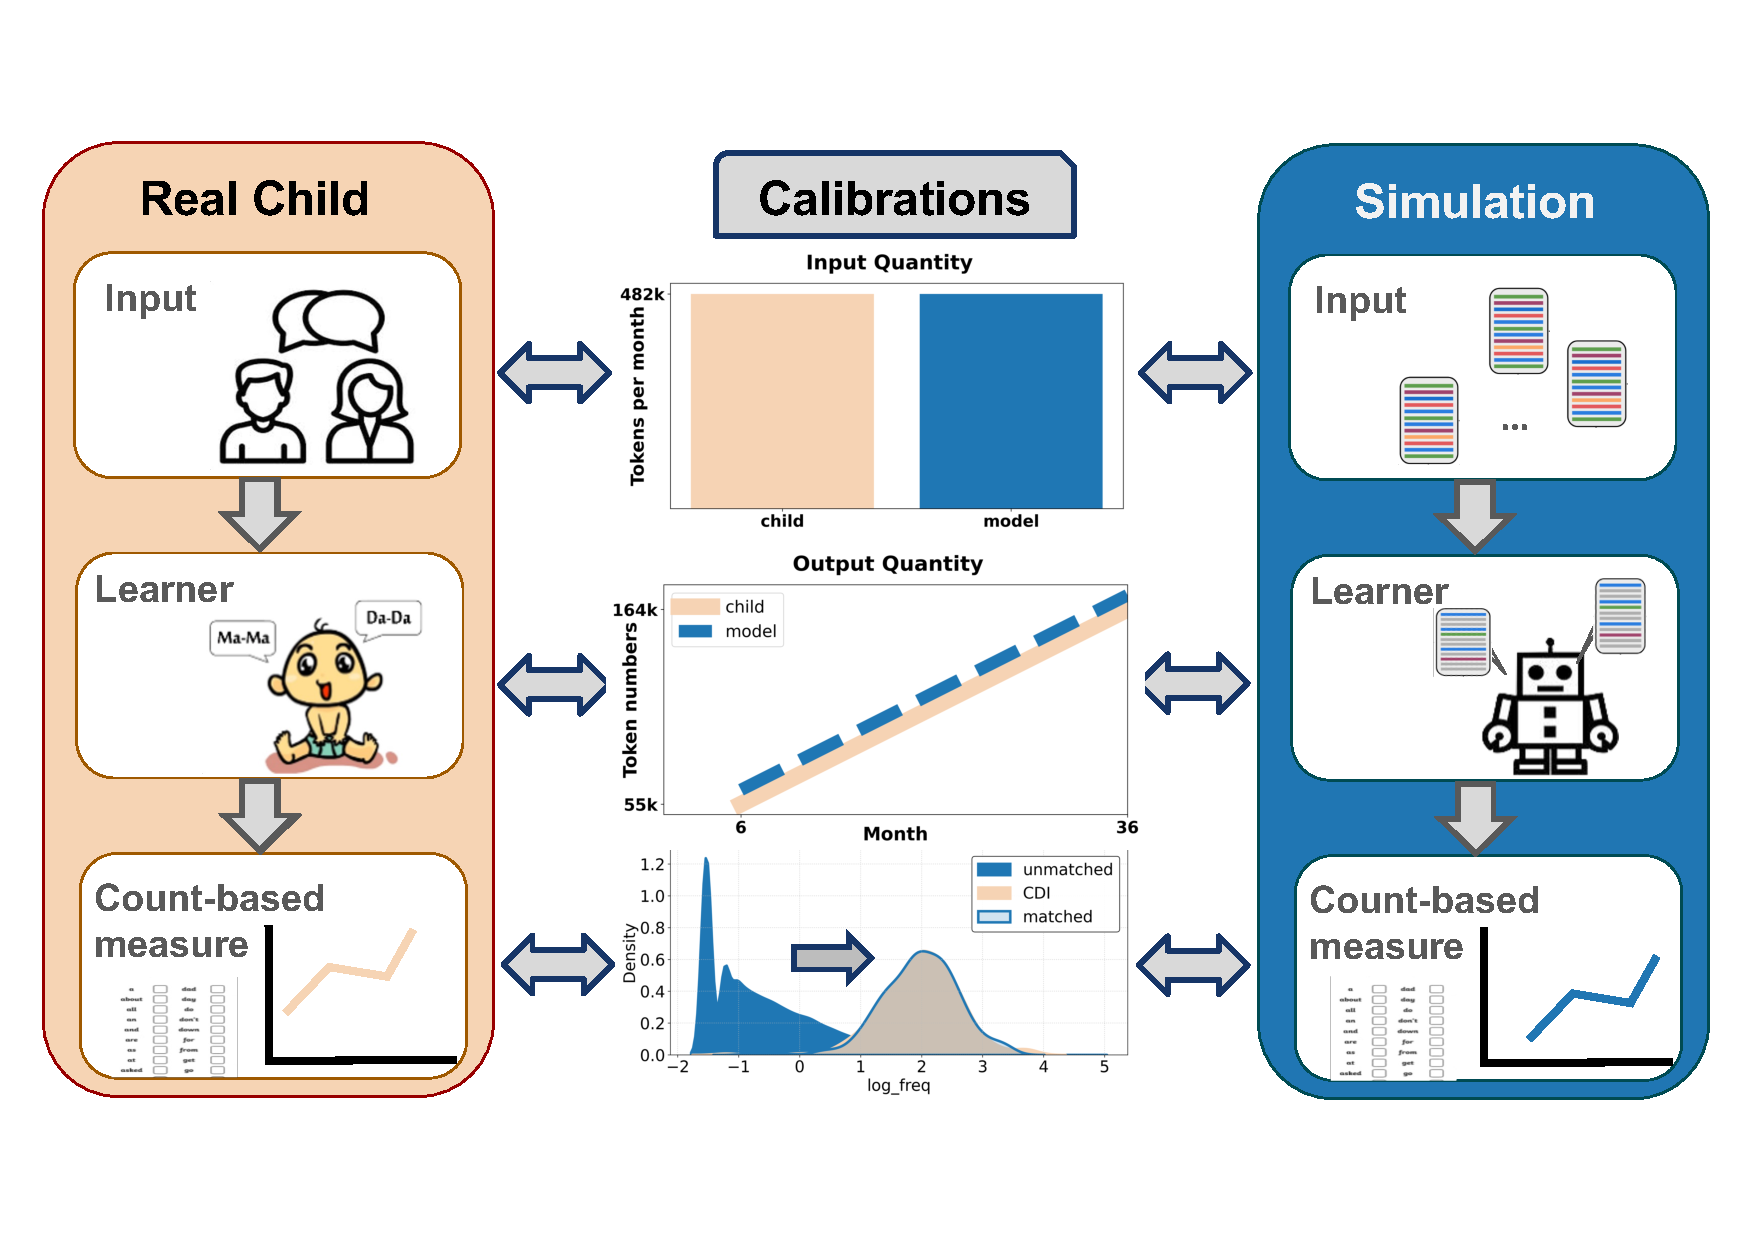
\includegraphics[width=0.5\textwidth]{fig/overview.pdf}}
\caption{\textbf{Overview of the \meCDI{} benchmark framework.} (a) Training and generation sizes are aligned with age-appropriate estimates of linguistic exposure and production from 6–36 months \citep{cristia2019child}. (b) Evaluation sets match the frequency distribution of MacArthur--Bates CDI words in child-directed speech (English-CHILDES).}
\label{fig:overview}
\end{figure}


\subsection{\meCDI{} Benchmark Overview}

The \meCDI{} benchmark enables direct comparison between language model generation and child production through three methodological calibrations to address common mismatches in prior work (Figure~\ref{fig:overview}):


\noindent\textbf{(1) Age-appropriate training exposure:} Training sets are scaled to match cumulative linguistic input from 6–36 months of age estimated from daylong recordings \citep{cristia2019child}.

\noindent\textbf{(2) Production quantity matching:} Generation sizes are calibrated to children's monthly word production rates estimated from longitudinal corpora \citep{cristia2019child} to ensure comparable sample sizes for vocabulary assessment.


\noindent\textbf{(3) Frequency-matched evaluation words:} The evaluation vocabulary is drawn from the MacArthur–Bates Communicative Development Inventory \citep{fenson2007macarthur} and frequency matched to words in English CHILDES corpora.  

We evaluate models on three dimensions: \textit{lexical diversity} (type–token ratio), \textit{word-form validity} (non-word rate), and \textit{target-word coverage} (\meCDI{} score).


\subsection{Training Data}

We construct two training corpora representing different linguistic environments:

\noindent\textbf{Audiobook corpus:} English audiobook transcripts from LibriVox \citep{kearns2014librivox}, representing narrative-rich, syntactically complex adult-directed language. \noindent\textbf{Child-directed speech (CDS) corpus:} English CHILDES transcripts \citep{macwhinney2000childes}, representing the naturalistic register of early child input.


\paragraph{Age-appropriate scaling} Following \citet{cristia2019child}, we estimate exposure from 250 hours at 6 months to 1,500 hours at 36 months of age. This corresponds to approximately 500 hours of speech input per year, representing a mid-range estimate of children's linguistic environments. The reported training budgets range from 2.89M words (6-month equivalent) to 17.35M words (36-month equivalent; Table~\ref{tab:train}).\footnote{The reported word budgets are not numerically identical to the originally reported conversion of three words per second. The conversion must be reconciled with the training records before these age-equivalent labels are used for precise estimates of developmental data efficiency.} Developmental datasets are constructed every 6 months by randomly sampling the target quantity from each corpus (see Table~\ref{tab:train}). Given English CHILDES contains a total of 15.6M words of caregiver inputs, the available data is equivalent to those at the 30-month level, which thus serves as the maximum training input. We emphasize that this scaling controls \emph{training-corpus size} rather than assuming uniform structure of children’s linguistic environments across months.



\paragraph{Preprocessing} All text is lowercased, with spaces and basic punctuation (periods, commas, apostrophes) preserved as word boundary markers. No subword tokenization is applied: models learn to generate word forms from character sequences while retaining these explicit orthographic boundary cues.

\subsection{Model Architectures and Training}

We train character-level autoregressive models under two architectures: \textbf{LSTM} Three layers with 200-dimensional character embeddings, 1024-dimensional hidden states, and 200-dimensional output projections, following \citet{lavechin2023babyslm}. \textbf{Transformer} GPT-2-style decoder-only architecture with 12 transformer layers, 512-dimensional hidden states, 12 attention heads per layer, following \citet{goriely2024babble}. 


\paragraph{Training procedure} Models are trained to minimize cross-entropy loss using the Adam optimizer (learning rate 0.0001, $\beta_1=0.9$, $\beta_2=0.98$) with inverse square root learning rate decay and 10,000 warmup steps. We train until validation perplexity converges. For each age-corpus pair, two models are trained with same random seeds and non-overlapping data subsets. Training details are provided in Table~\ref{tab:model}.


\paragraph{Generation procedure} At inference time, we generate text using temperature sampling with $T \in \{0.3, 0.6, 1.0, 1.5\}$. Generation begins with a beginning-of-sequence (BOS) token and continues until reaching the target word count corresponding to children's estimated monthly production at that developmental stage (see Table~\ref{tab:speech-metrics} in Appendix). Character sequences are segmented into words using space and punctuation boundaries. Because the CDS corpus contains a total of 15.6M words of caregiver input, this limits the age-appropriate training to the 30-month equivalent. In the CDS conditions, for months 31–36 we generate outputs using the same 30-month checkpoint, scaling generation lengths according to children’s estimated production, while noting that the training exposure does not increase beyond 30 months. These later points change the observation budget without adding training material; they therefore cannot be interpreted as further learning from additional input.
% AUTHOR CHECK: confirm whether checkpoint reuse after month 30 applies to every corpus or only CDS, and specify checkpoint assignment between six-month training targets.


\subsection{Evaluation Set Construction} \label{sec:eval_construction}
\paragraph{Base vocabulary and POS filtering} We start with the MacArthur--Bates Communicative Development Inventories (CDI) \citep{fenson2007macarthur}, a standardized checklist of 680 English words with normative age-of-production data. To control for lexical class effects, we apply POS tagging using a RoBERTa-based SpaCy pipeline. For each word, POS labels are aggregated across contexts and majority voting is applied separately in each corpus. Function words (articles, pronouns, prepositions, auxiliaries) are excluded, retaining nouns, verbs, adjectives, and adverbs.

\paragraph{Frequency stratification} Filtered CDI words are divided into six frequency bands based on their occurrence in child-directed speech (adult input in English CHILDES), with an equal number of words per band. 

\paragraph{Audiobook subset selection}

For a comparable evaluation, we construct a matched audiobook subset using the same POS filtering and frequency banding. Words are selected such that their frequency distribution mirrors the filtered CDI evaluation set. This process yields two aligned datasets: i.) Filtered CDI evaluation set with 420 words in six frequency bands; and ii.) frequency-matched audiobook subset with the same size per frequency band. This enables a developmentally grounded comparison between model generations and children’s expressive vocabulary.



\subsection{Evaluation Metrics}

We assess model performance using three complementary metrics capturing lexical diversity, word-form validity, and target-word coverage.


\paragraph{Type-Token Ratio (TTR)} Measures lexical diversity as the ratio of unique word types to total word tokens. Following \citet{rasanen2024age}, we compute TTR over fixed-size chunks of 3,500 words to control for sample size effects, then average across all chunks.

\paragraph{Non-word Rate} Quantifies word-form validity as the proportion of generated word types not found in the reference lexical resources: CELEX, the Enchant library,\footnote{\url{https://pypi.org/project/pyenchant/}} and Wiktionary.\footnote{\url{https://www.wiktionary.org}} A word is classified as valid if it appears in any of these resources. This is an orthographic dictionary-membership measure, not a direct measure of speech accuracy or contextual appropriateness.
% AUTHOR CHECK: verify the exact lexical resources and versions. The previous CELEX citation key van2014subtlex refers to SUBTLEX-UK.


\paragraph{\meCDI{} Score} Adapts the human CDI vocabulary assessment to observed productions through a count-based criterion. A word meets the production criterion if it appears at least $\tau$ times in the evaluated output. To determine $\tau$, we compare vocabulary growth curves derived from CHILDES child productions with the empirical CDI trajectory. We use $\tau = 60$, selected on the basis of the reported slope comparison. This is a calibration rule linking corpus counts to caregiver reports, rather than an independent test of lexical knowledge. The \meCDI{} score is computed as:
$$
\text{\meCDI{}} = \frac{|\{w \in \text{eval set} : \text{count}(w) \geq \tau\}|}{|\text{eval set}|}
$$
where the evaluation set contains 420 target words. The value represents the proportion of that set reaching the count criterion under the specified production budget. Sensitivity analyses for alternative thresholds ($\tau \in \{1, 500\}$) are shown in Figure~\ref{fig:threshold}.
% AUTHOR CHECK: specify whether counts are monthly or cumulative across months, how child transcripts are pooled, the calibration objective, and whether calibration and final evaluation are independent.





\section{Results}

\begin{figure*}[!htp]
\centering
\subfloat{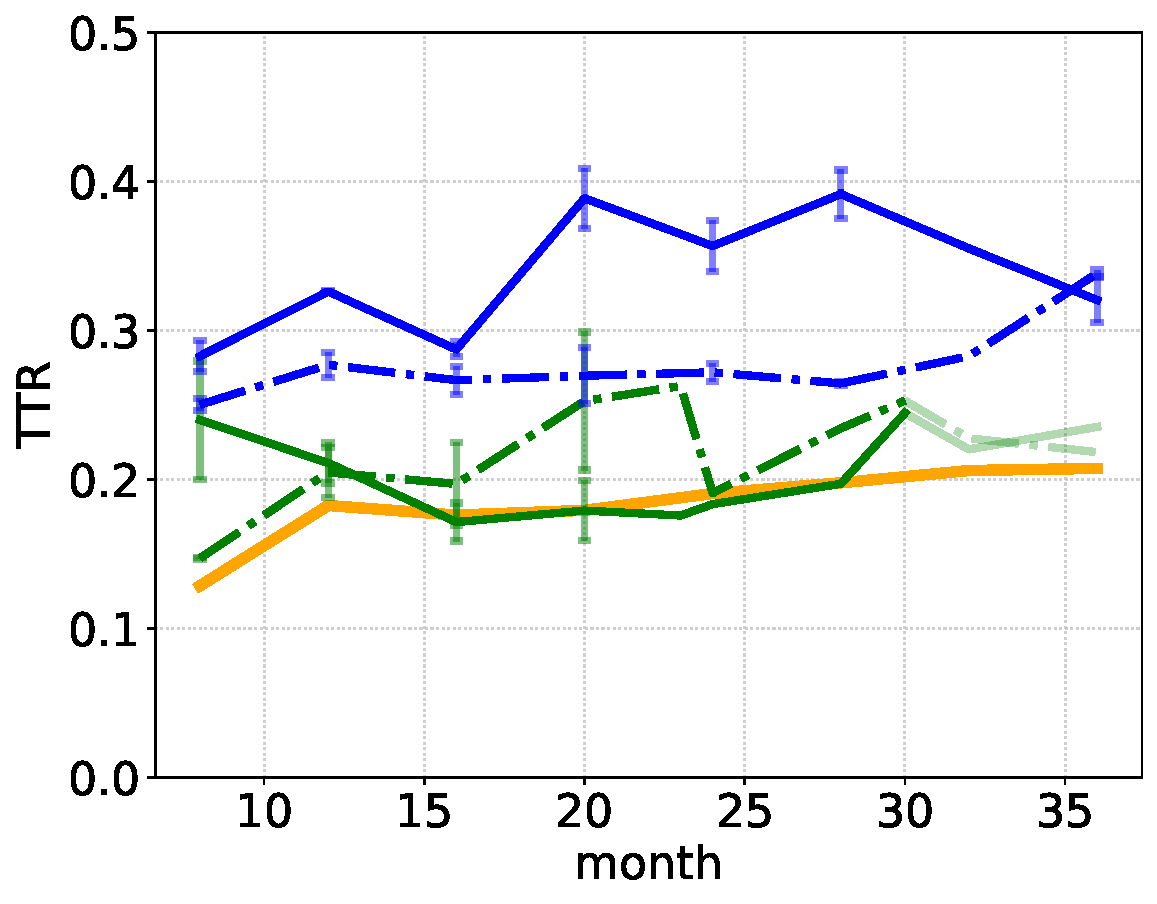
\includegraphics[width=0.27\textwidth]{fig/ttr_500_1.pdf}}
\hspace{2pt}
\subfloat{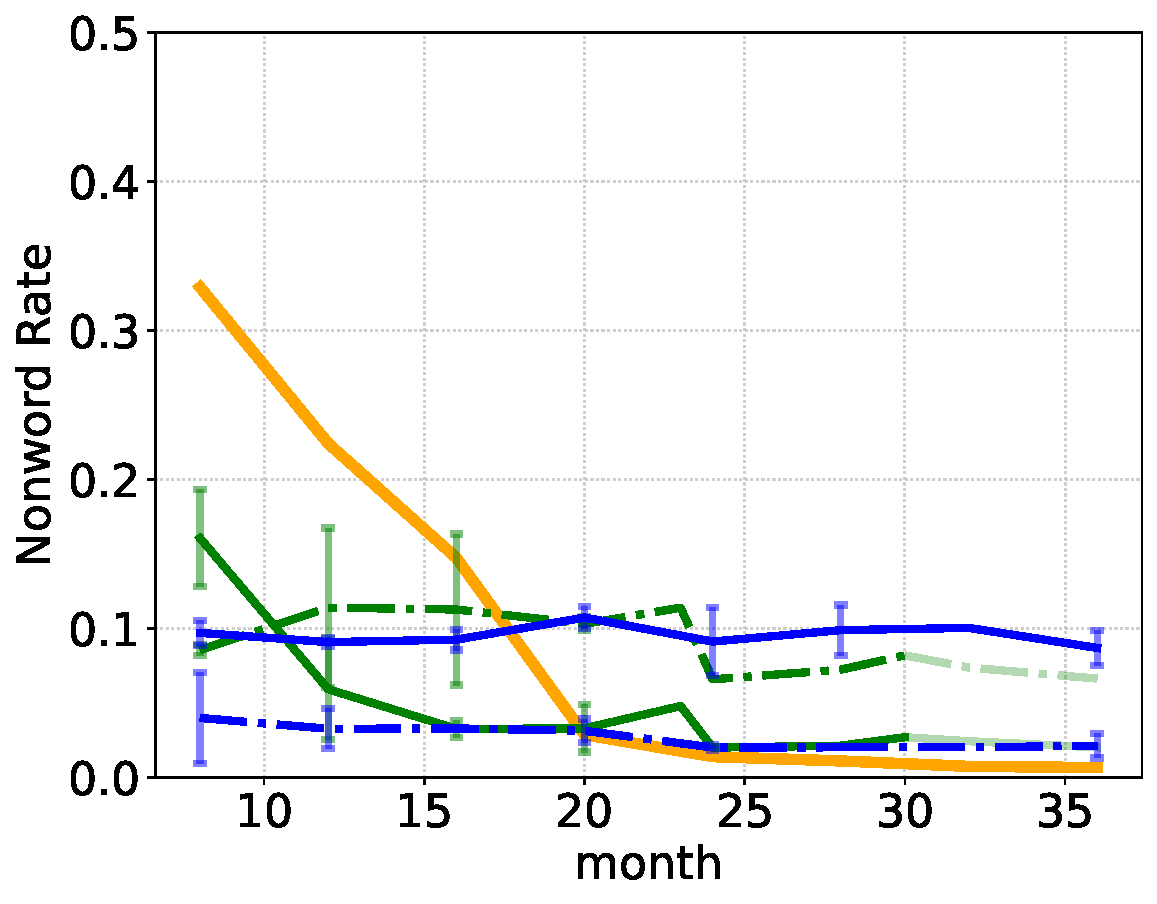
\includegraphics[width=0.27\textwidth]{fig/Nonword Rate_500_1.pdf}}
\hspace{2pt}
\subfloat{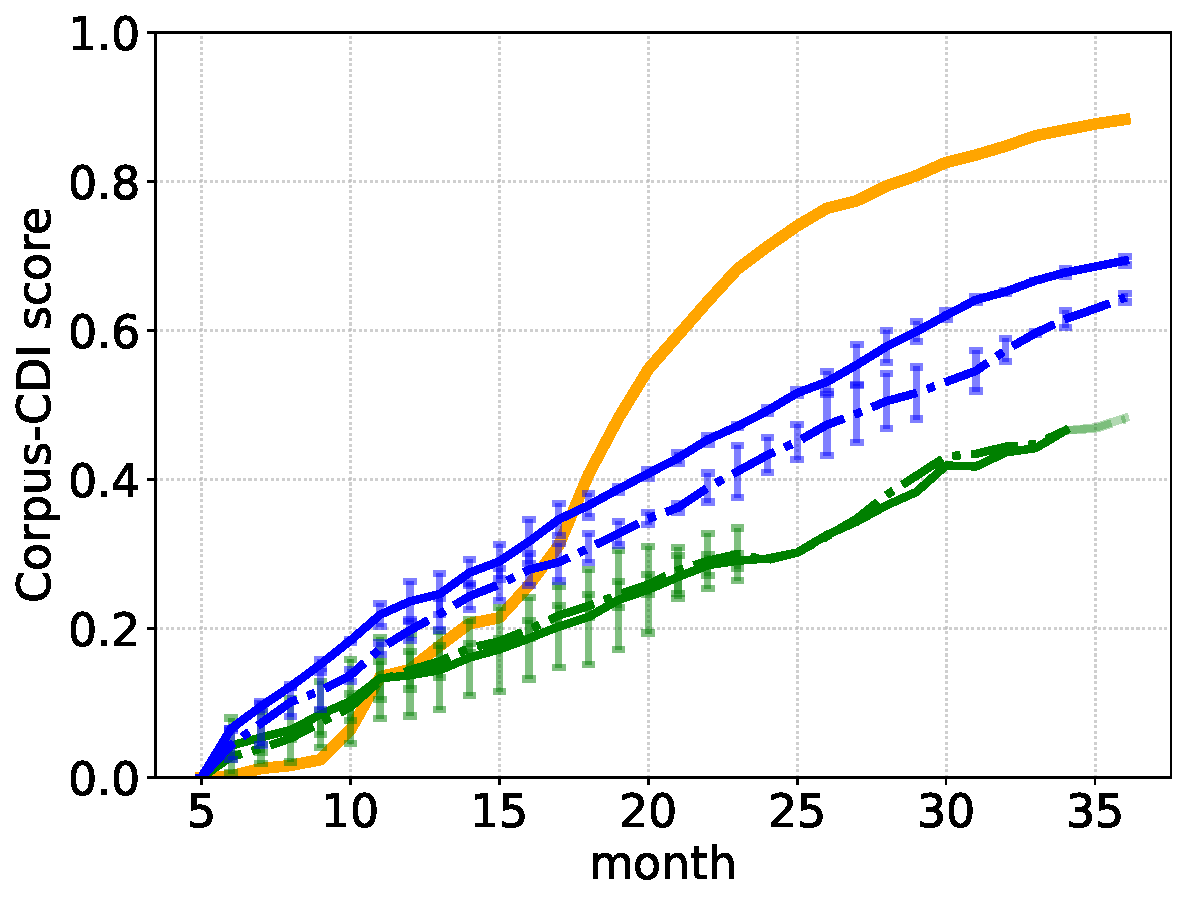
\includegraphics[width=0.27\textwidth]{fig/Corpus-CDI score_500_1.pdf}}
\hspace{2pt}
\subfloat{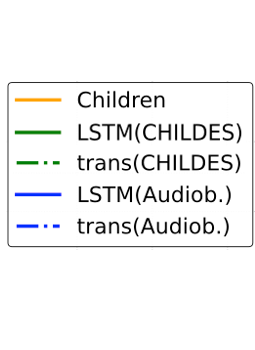
\includegraphics[width=0.13\textwidth]{fig/legend.png}}
\caption{\textbf{Core metrics comparing child and model vocabulary development across age groups.} Left: type--token ratio (TTR). Middle: non-word type rate under dictionary matching. Right: \meCDI{} coverage, with words counted when produced at least 60 times. Results are shown for LSTM and Transformer models trained on audiobooks and child-directed speech (CDS), compared with CHILDES child production data. Error bars are reported as 95\% confidence intervals across training subsets. The lighter CDS points after the 30-month-equivalent checkpoint use increasing output budgets without additional training input.}
% AUTHOR CHECK: verify the confidence-interval procedure and its independent sampling units.
\label{fig:core_metric}
\end{figure*}





\begin{figure*}[!ht]
\centering
\subfloat{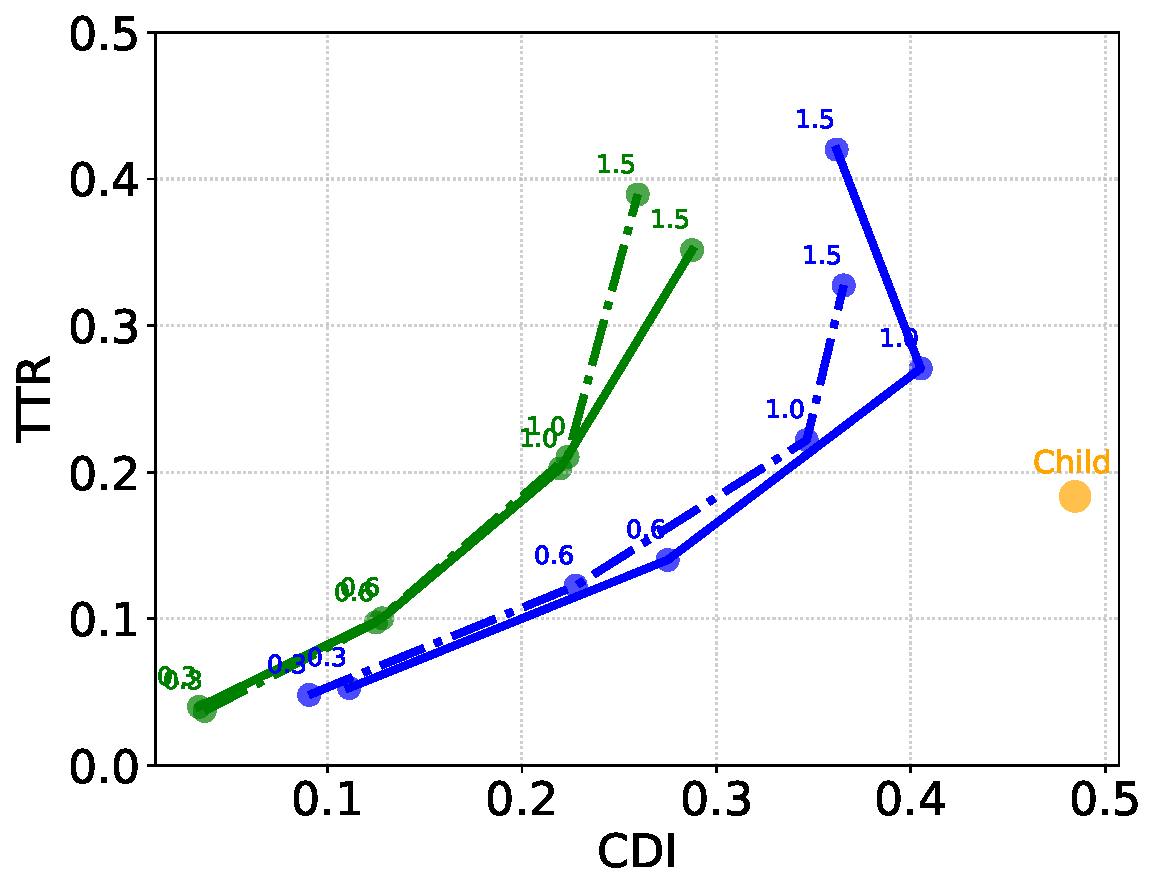
\includegraphics[width=0.35\textwidth]{fig/temp_ttr_500_1.pdf}}
\hspace{2pt}
\subfloat{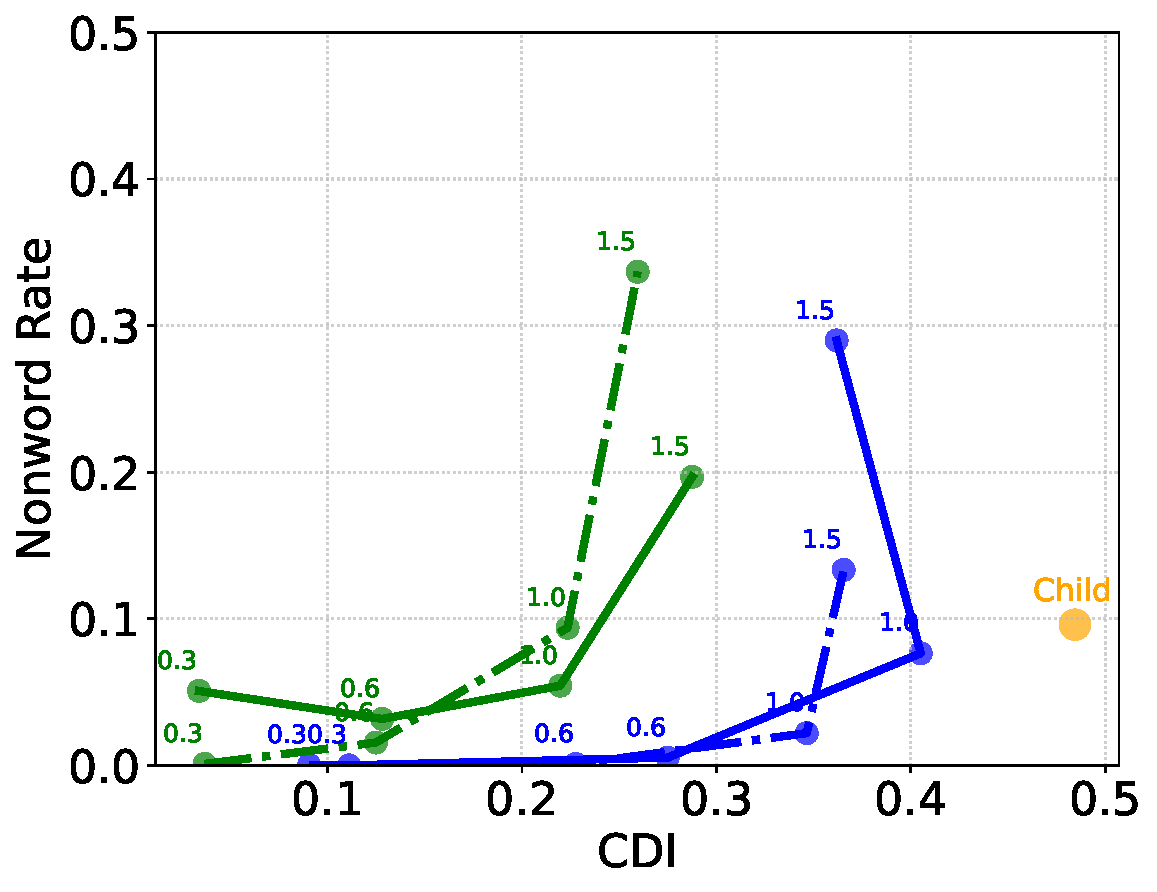
\includegraphics[width=0.35\textwidth]{fig/temp_Nonword Rate_500_1.pdf}}
\hspace{2pt}
\hspace{2pt}
\subfloat{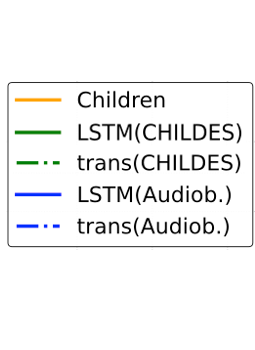
\includegraphics[width=0.13\textwidth]{fig/legend.png}}
\caption{\textbf{Temperature trade-off across different metrics; temperature settings (0.3-1.5)} Left: Trade-off between type-token ratio and CDI score. Right: Relationship between non-word rate and CDI score.  Each point averages across the evaluated exposure stages for one architecture, corpus, and temperature; numbers identify the temperature.}
\label{fig:temp_effect}
\end{figure*}





 
\subsection{Developmental Trajectories}
\label{sec:trajectories}

Figure~\ref{fig:core_metric} presents three production measures against developmental labels derived from estimated input and output quantities, alongside the CHILDES child reference. All results use temperature $T=1.0$ as the default setting. The later CDS points retain the same training checkpoint and vary the production budget, as described in the generation procedure.

\paragraph{Lexical diversity} Audiobook-trained models exhibit higher type-token ratios than the child reference across the plotted stages. CDS-trained models are closer to the child values at several stages, with differences depending on architecture and input scale. The child TTR rises overall, whereas model curves show condition-specific fluctuations rather than a common developmental trend. Thus lexical diversity distinguishes input registers and model conditions, but does not imply that every model consistently exceeds the child reference.


\paragraph{Word-form validity} The proportion of child word types absent from the reference dictionaries decreases markedly with age. Model trajectories vary: several are relatively flat, whereas the CDS-trained LSTM shows a substantial decline. No single model curve reproduces the full child pattern across the plotted range. Because this measure is computed from written forms, it cannot identify the contribution of children's articulatory or phonological development separately from transcription and dictionary coverage.



\paragraph{Vocabulary growth} The child \meCDI{} trajectory contains a pronounced period of accelerated growth, followed by a slower rise. Model coverage also increases, but follows a more nearly linear pattern over the observed range. Audiobook-trained models achieve greater coverage than CDS-trained models in the figure, although their evaluation sets are frequency-matched rather than lexically identical. The main comparison concerns the differing trajectory shapes; a universal ranking of the architectures is not supported by these curves.

Taken together, the measures show that the tested models do not jointly reproduce the child production profile. The vocabulary-coverage discrepancy appears across architectures and corpora, while the magnitude and direction of TTR and non-word differences depend on condition. The next analyses test whether the sampled decoding temperatures improve this joint alignment (Section~\ref{sec:temperature}) and how the coverage discrepancy varies with lexical frequency (Section~\ref{sec:frequency}).


\subsection{Temperature Tradeoff} 
\label{sec:temperature}

The developmental gaps observed in Section~\ref{sec:trajectories} raise an important question: could these differences arise from suboptimal generation parameters rather than inherent learning limitations? Temperature sampling controls generation stochasticity, with lower temperatures favoring high-probability outputs and higher temperatures increasing diversity. We evaluate whether any temperature setting can align models with children across all three metrics.

Figure~\ref{fig:temp_effect} shows the relationships between metrics as temperature varies from 0.3 to 1.5. Each point represents the mean performance across all developmental stages for a given architecture, corpus, and temperature combination.

\paragraph{TTR-CDI trade-off} Temperature changes the relation between lexical diversity and target-word coverage. Lower temperatures concentrate output on fewer forms, whereas higher temperatures increase diversity. Coverage does not increase monotonically in every condition: in the audiobook models it declines between $T=1.0$ and $T=1.5$, even as TTR increases. None of the tested settings jointly matches the child reference on TTR and \meCDI{} coverage. Thus this temperature manipulation does not resolve the observed discrepancy between lexical variety and repeated production of target words.


\paragraph{Non-word-CDI trade-off} High temperatures generally increase non-word rates, with the pattern depending on architecture and corpus. Some conditions approach the child's mean non-word rate without matching its vocabulary coverage. Moreover, similar means can summarize different developmental trajectories, as shown in Figure~\ref{fig:core_metric}. Alignment on this single aggregate measure therefore does not establish alignment of the overall production profile.


Within the tested temperature range, decoding changes do not remove the joint discrepancy between child and model production measures. This rules out a particular adjustment as a sufficient explanation of the result, while leaving open other decoding, elicitation, and learning procedures. The next section examines the relation between the coverage discrepancy and input frequency.



\subsection{Frequency effect} 
\label{sec:frequency}

\begin{figure}[!h]
\centering
\adjustbox{trim={30 20 30 20}, clip}{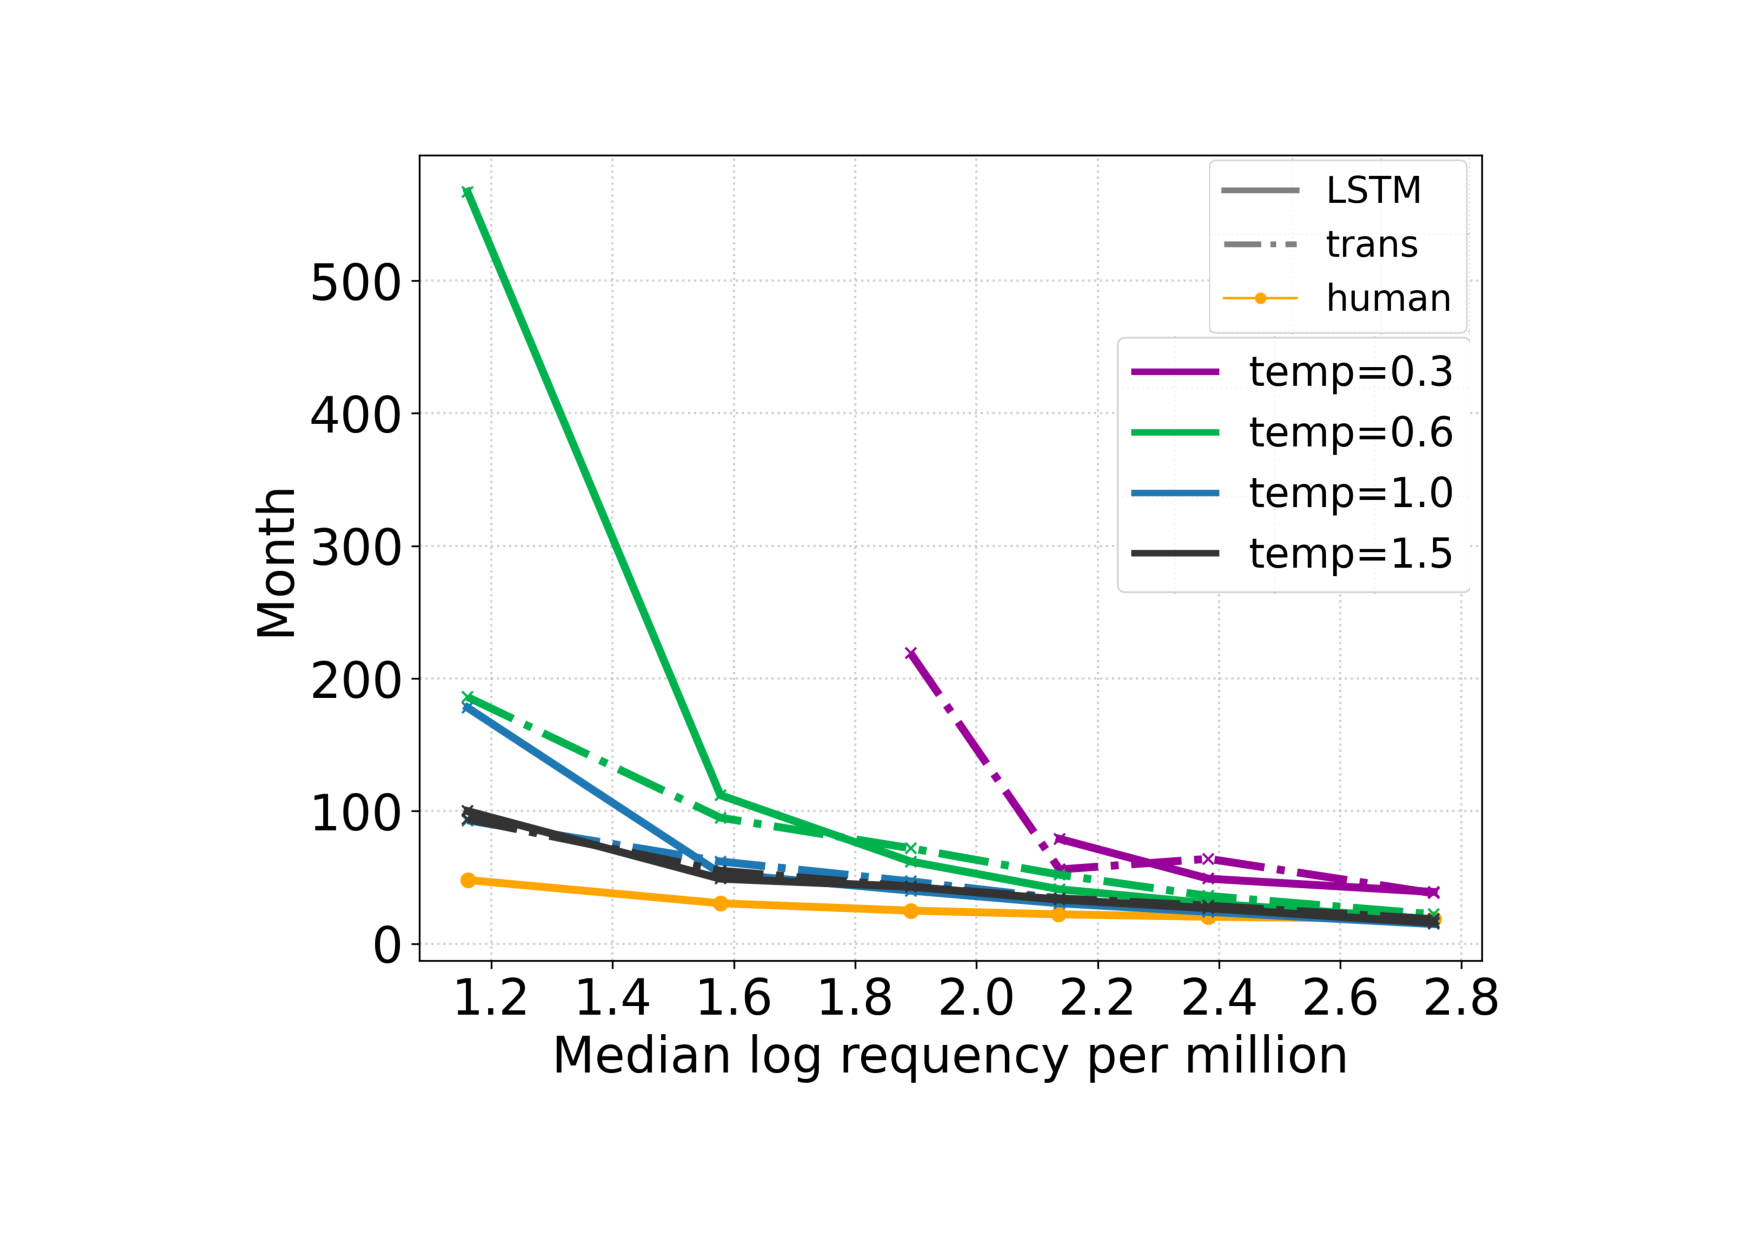
\includegraphics[width=0.6\textwidth]{fig/freq_stela.pdf}}
\caption{\textbf{Fitted criterion-crossing months by frequency band for audiobook-trained models and the child reference.} The horizontal axis gives median log frequency per million; the vertical axis gives the month at which the fitted trajectory reaches 80\% coverage within the band. Values beyond the observed age or exposure range are extrapolations, not observed training requirements. Missing model points indicate that no criterion-crossing estimate is reported for that condition.}
% AUTHOR CHECK: document the fitting equation, observed fitting range, uncertainty and reason for missing estimates.
\label{fig:freq_effect}
\end{figure}


We next examine whether the vocabulary-coverage discrepancy is uniform across frequency. The evaluation sets are divided into six bands, and sigmoid curves are fitted to the proportion of words meeting the count criterion in each band. A criterion-crossing month is extracted where a fitted curve reaches 80\% coverage. This summarizes the fitted relation between frequency and production, conditional on the exposure and output scaling. Estimates outside the observed range are extrapolations, including any child-reference estimates beyond the ages represented in the data.
% AUTHOR CHECK: provide the sigmoid equation, fitting parameters and constraints, observed fitting range, and handling of absent or unstable crossings.


\paragraph{Divergent frequency sensitivity} Figure~\ref{fig:freq_effect} shows a steeper relation between frequency and fitted criterion-crossing time for the models than for the child reference, especially in the lowest-frequency band. Model estimates also vary substantially with temperature. At high frequencies, several model estimates approach the child estimate. The result identifies frequency-dependent difficulty in meeting this production criterion; it does not directly measure how much input is necessary for a word to be represented or understood.


\paragraph{Temperature modulation} Temperature modulates the frequency pattern. At $T=0.3$, sampling is concentrated on high-probability continuations, and some low-frequency bands have no reported criterion-crossing estimate. Higher temperatures make additional forms available in generation, although lower-frequency model estimates remain especially sensitive to condition. Because the count criterion depends on generated occurrences, this analysis reflects both what the trained model assigns probability to and how that probability is sampled.


\paragraph{Long-tail truncation} The frequency pattern is consistent with underproduction of forms in the lexical long tail. In empirical cross-entropy training, frequent events contribute repeatedly to the aggregate training signal. During finite generation, low-probability forms also have fewer opportunities to accumulate enough occurrences to pass a fixed count threshold. Together, these factors provide a plausible account of the observed production pattern. The present design does not isolate the objective from representation, corpus composition, optimization, or decoding, and does not establish that representational capacity is allocated in direct proportion to word frequency.


Evidence from child word learning motivates possible additional sources of support, including memory for particular learning events \citep{markson1997evidence}, cross-situational information \citep{smith2008infants}, and social-pragmatic cues \citep{tomasello2000social}. These possibilities suggest interventions for subsequent modeling work. They are not manipulated here, so the current results cannot determine which resource explains the child--model production discrepancy or exclude a contribution from predictive learning in children.


\subsection{Production of Content Words}
\label{sec:content_word}


\begin{figure}[!h]
\centering
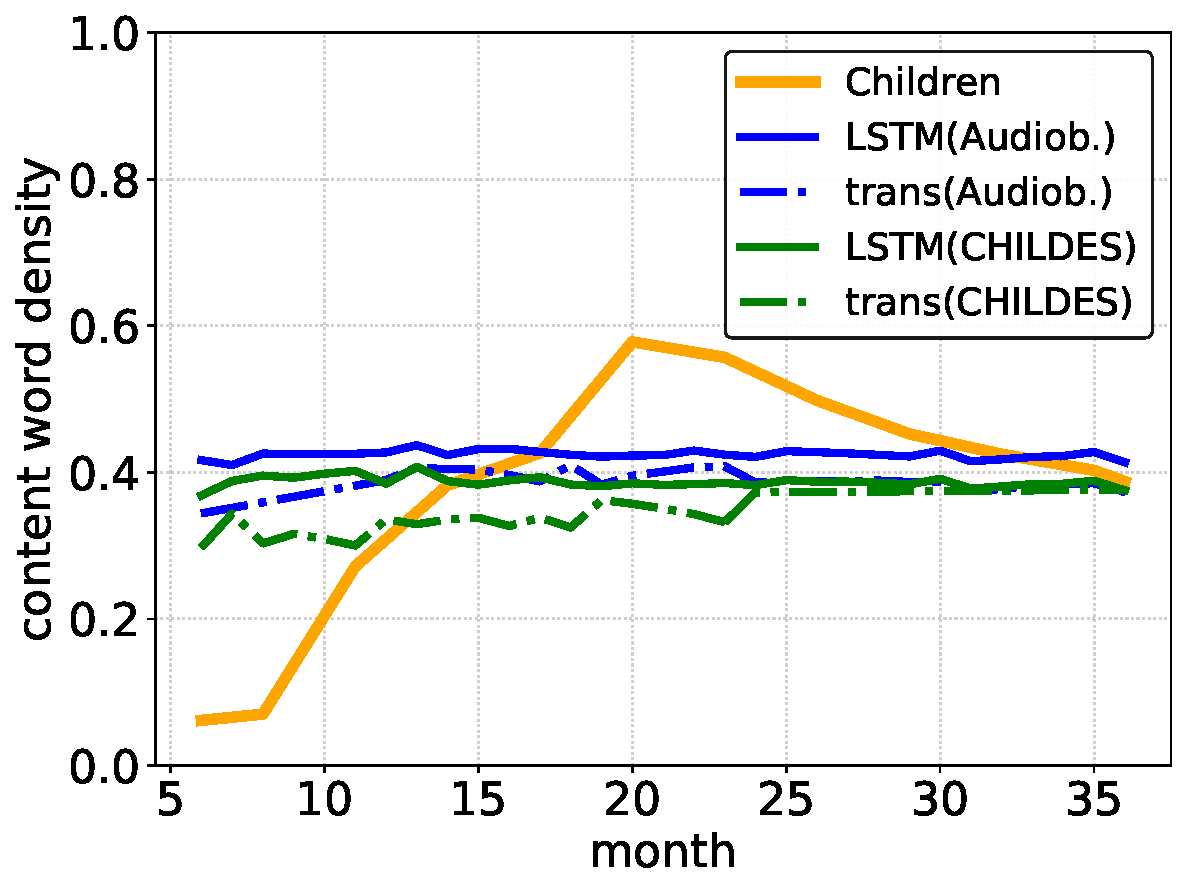
\includegraphics[width=0.48\textwidth]{fig/content_500_1.pdf}
\caption{\textbf{Proportion of content words in generated text across development.} Children show an inverse U-shaped trajectory, while model proportions occupy a narrower range, generally around 40\%, with some variation across training stages.}
\label{fig:content_prop}
\end{figure}


The frequency-dependent pattern in Section~\ref{sec:frequency} motivates examining the allocation of output to content and function words. The \meCDI{} evaluation targets content words (Section~\ref{sec:eval_construction}), whereas TTR is calculated over the sampled vocabulary more broadly. A model can therefore have a high overall TTR without repeatedly generating enough target content words to attain high \meCDI{} coverage.


\paragraph{Children's inverse U-shaped trajectory} Figure~\ref{fig:content_prop} shows a pronounced rise and subsequent fall in the proportion of content words in child productions. This is consistent with a changing lexical composition as vocabulary expands and grammatical function words become more prevalent \citep{bates1994developmental,brown1973first}. Coverage of the target vocabulary continues to increase while its share of all produced tokens declines, illustrating that vocabulary coverage and token allocation measure different properties.

\paragraph{Models' narrower range}

Model content-word proportions vary within a narrower range, generally around 40\%, although some conditions change with training scale. The models do not show the pronounced peak present in the child curve. This establishes a distributional difference without requiring the assumption that model output is identical to an adult corpus distribution.

The joint analysis shows that target-word coverage, lexical diversity, and lexical-category proportions need not move together. The content-word pattern is relevant to interpreting coverage on a content-word evaluation set, but it does not by itself explain the cause of elevated TTR or establish that function-word production displaces particular target words.

These observations extend the trajectory comparison from the number of target words produced to the distribution of output across lexical categories. Testing why those distributions differ would require controlled changes to the learning or production procedure.



% Candidate thesis discussion. Prefer replacing the paper's existing Discussion
% section (baseline lines 312--326); retain its Methods, Results and Limitations.
\section{Chapter discussion}
\label{sec:ch3:chapter-discussion}

\subsection{What the comparison establishes}

This chapter makes expressive production an explicit target for developmental comparison. The main empirical finding is a discrepancy in the joint pattern of vocabulary coverage, lexical diversity, and word-form validity. With larger training corpora, models produce more of the evaluation vocabulary often enough to cross the \meCDI{} threshold. They nevertheless fail to reproduce the accelerated middle portion of the child corpus trajectory. This mismatch is visible across the tested architectures and input registers, although individual measures vary across conditions: audiobook-trained models have especially high lexical diversity, whereas some child-directed-speech conditions approach children's TTR or show substantial declines in non-word production (Figure~\ref{fig:core_metric}). The result is therefore a constraint on the overall production profile, rather than evidence that every model is equally distant from children on every measure.

The temperature experiment strengthens this conclusion by testing one concrete alternative explanation. Among the sampled temperatures, moving toward more diverse output does not yield a configuration that jointly matches the child reference on vocabulary coverage and TTR (Figure~\ref{fig:temp_effect}). It can also increase the rate of forms absent from the reference dictionaries. This is a useful robustness result: the discrepancy is not removed by choosing another value within the tested temperature range. It leaves open whether other elicitation contexts, decoding policies, or training procedures would produce a different relation among the measures.

\subsection{Measurement, benchmark, and model contributions}

The measurement contribution is to specify the observation process through which a vocabulary estimate is obtained. Fixed-size windows make TTR less dependent on the amount of sampled text; production budgets define opportunities to observe words; and the count threshold defines how much observed evidence is required for an item to contribute to the vocabulary score. The benchmark contribution is to combine these decisions with explicit input scales and frequency-matched evaluation sets, allowing a common protocol to be applied to two architectures and two registers. The model comparison then provides empirical constraints on those particular learners under that protocol. These contributions remain useful even when a numerical score cannot be read as an inventory of everything a learner knows.

The distinction matters especially for \meCDI{}. Its threshold was chosen by comparing child corpus counts with a caregiver-report trajectory. This calibration supplies a linking rule between measurements; agreement on the calibration material is not independent validation of lexical knowledge. A target form may remain below threshold because it is weakly represented, because relevant contexts are rarely sampled, or because more probable alternatives occupy the generated output. Conversely, frequent production alone does not establish appropriate reference or contextual use. A stronger validation would apply the fixed calibration to held-out children or corpora and test whether the resulting estimates agree with additional vocabulary measures. The present score is most directly interpretable as the proportion of target forms reaching a production criterion under the specified sampling conditions.

\subsection{Frequency and the meaning of data efficiency}

Frequency analysis identifies where the production discrepancy is largest. The fitted trajectories are more frequency-sensitive for the evaluated models than for the child reference, particularly in the lower-frequency bands (Figure~\ref{fig:freq_effect}). The associated content-word analysis adds an informative distributional difference: the child corpus shows a pronounced rise and subsequent fall in content-word proportion, whereas the model proportions vary within a much narrower range (Figure~\ref{fig:content_prop}). Thus vocabulary coverage and the distribution of output across lexical categories need to be considered together. A model can generate many distinct forms while repeatedly producing too few of the particular content words scored by the benchmark.

This pattern is compatible with an interaction between frequency-weighted predictive training and finite sampling. Under an empirical cross-entropy objective, frequent events contribute repeatedly to the training signal. During generation, low-probability forms also have fewer opportunities to accumulate enough occurrences to pass a fixed count threshold. These considerations motivate the hypothesis that the tested learning and production procedures provide insufficient support for parts of the lexical long tail. The experiment does not isolate the objective as the unique cause: it does not compare cross-entropy with another objective while holding the remaining conditions fixed. Likewise, the content-word proportions do not by themselves identify a causal explanation for TTR. The results locate a frequency-related discrepancy and define hypotheses that can be tested through interventions on memory, objectives, input, or production.

The time axis further limits a numerical claim about data efficiency. Model conditions vary in available corpus size and are trained to convergence, so the amount of distinct text is not the total number of word presentations during optimization. The age-equivalent scale also combines estimated input with increasing output budgets. In the CHILDES conditions, the available training corpus limits further input growth after the 30-month-equivalent checkpoint, while later generation budgets continue to change. Those later observations cannot therefore be attributed wholly to additional learning. Finally, frequency-band estimates that cross the acquisition criterion far beyond the observed range are curve extrapolations, not results from models actually trained on hundreds of months of input. Their magnitude depends on the fitted function and threshold. Within these boundaries, the study shows that increasing corpus size under the tested protocol does not automatically recover the child production profile; it does not determine a universal child--model data multiplier.

\subsection{From a diagnostic discrepancy to a controlled intervention}

The strongest next step is to preserve the production measure while manipulating a candidate source of the discrepancy. An episodic store could test whether access to particular encounters improves low-frequency target coverage; alternative training objectives could test whether changing the weighting of rare events changes that coverage; and grounded or interactive input could test whether referential and conversational context changes which words are produced. Such comparisons should count any additional information and evaluate effects across multiple outcomes, since an improvement in thresholded coverage could coexist with deteriorating lexical diversity or word-form validity.

Chapter~\ref{chp3_chap} takes up one related intervention by asking whether retrieval of stored linguistic instances improves sensitivity to low-frequency syntactic contrasts. It tests the potential contribution of instance-based access using a different outcome and experimental setting. It consequently extends the inquiry into sparse evidence without directly repairing or explaining the expressive-vocabulary curves reported here. Across the two studies, the common question is what information remains available to a predictive learner when relevant evidence is infrequent, and how that availability depends on the task used to measure it.



 
\section{Limitations}

Our evaluation framework has several limitations. First, we evaluate character-level models rather than speech-based systems. Character input supplies stable orthographic forms and explicit boundaries, bypassing acoustic variability and aspects of segmentation \citep{dupoux2018cognitive}. Speech-based language models \citep{lakhotia2021generative,nguyen2024spirit} face a different representation problem. The direction and magnitude of a child--model gap under speech input cannot be established from the present comparison. Extending \meCDI{} to speech would require a validated mapping from acoustic output to the forms used for vocabulary scoring. The models also lack the multimodal and interactive information available in children's environments, whose contribution is not isolated here.

Second, the CHILDES transcripts used as reference data introduce possible biases. Adult transcription and normalization can change which child forms are recorded and whether they match reference dictionaries. A dictionary-based non-word score therefore combines properties of the child's production, transcription choices, and lexical-resource coverage. Character-level model output can be assessed directly as written forms, but the model can still generate non-words; this does not supply an equivalent measure of children's spoken production accuracy.


Third, caregiver CDI reports and counts in generated text are related but distinct measurements. A report that a child says a word summarizes observations across contexts; \meCDI{} applies a frequency criterion to a sampled output. Neither one occurrence nor repeated occurrences alone establishes the full meaning or appropriate use of a word. The threshold ($\tau = 60$) calibrates the corpus measure against the reference trajectory, but its construct validity requires further testing on independent materials and outcomes.


Finally, our study focuses on English and a single vocabulary assessment tool (CDI). Cross-linguistic validation is essential for establishing universality: languages with richer morphology, less transparent orthography, or different child-directed registers may yield different alignments between model and child learning. Character-level models in particular may be sensitive to orthographic properties, limiting generalizability beyond English.


\section{Ethics Statement}

The study uses existing CHILDES child-language data, LibriVox audiobook transcripts, and CDI vocabulary reference materials. Its purpose is model benchmarking and research on language acquisition. These evaluations do not establish suitability for real-world deployment. Any reuse of the source materials should follow the applicable access and data-use conditions.
% AUTHOR CHECK: confirm the exact data versions, access conditions, and any required ethics or consent statement; no new human-data collection or approval is asserted here.



% \section*{Acknowledgments}
% add erc affiliations from the template

% Bibliography entries for the entire Anthology, followed by custom entries
%\bibliography{anthology,custom}
% Custom bibliography entries only
%\newpage

\newpage

\section{Appendix}

\subsection{Training and generation details}

Table~\ref{tab:train} summarizes the age-appropriate scaling of training data across three exposure scenarios. Linguistic exposure estimates are based on daylong recording studies \citep{cristia2019child}, which document substantial variability in the amount of speech heard by children across environments. Annual exposure ranges from approximately 100 hours in low-input households to 1000 hours in high-input ones, with 500 hours per year representing a mid-range estimate.

Cumulative exposure thus increases from 50–500 hours at 6 months to 300–3000 hours by 36 months. The reported word budgets range from 0.58M words (6 months, low exposure) to 34.71M words (36 months, high exposure).


\begin{table}[ht]
\centering
\small
\begin{tabular}{l c c c c}
\toprule
\textbf{Age (mo.)} & \textbf{Hours} & \textbf{Words (M)} & \textbf{Chars. (M)} & \textbf{Utts. (k)} \\

\midrule
\multicolumn{5}{l}{\textit{Low exposure scenario (100 hours/year)}} \\
\midrule
6   & 50   & 0.58  & 2.95  & 58   \\
12  & 100  & 1.16  & 5.89  & 116  \\
18  & 150  & 1.73  & 8.84  & 173  \\
24  & 200  & 2.31  & 11.78 & 231  \\
30  & 250  & 2.89  & 14.73 & 289  \\
36  & 300  & 3.47  & 17.67 & 347  \\
\midrule
\multicolumn{5}{l}{\textit{Medium exposure scenario (500 hours/year)}} \\
\midrule
6   & 250  & 2.89  & 14.73 & 289  \\
12  & 500  & 5.78  & 29.45 & 578  \\
18  & 750  & 8.68  & 44.18 & 868  \\
24  & 1000 & 11.57 & 58.90 & 1157 \\
30  & 1250 & 14.46 & 73.63 & 1446 \\
36  & 1500 & 17.35 & 88.35 & 1735 \\
\midrule
\multicolumn{5}{l}{\textit{High exposure scenario (1000 hours/year)}} \\
\midrule
6   & 500  & 5.78  & 29.45 & 578  \\
12  & 1000 & 11.57 & 58.90 & 1157 \\
18  & 1500 & 17.35 & 88.35 & 1735 \\
24  & 2000 & 23.14 & 117.80 & 2314 \\
30  & 2500 & 28.92 & 147.25 & 2892 \\
36  & 3000 & 34.71 & 176.70 & 3471 \\
\bottomrule
\end{tabular}
\caption{\textbf{Age-appropriate scaling of training datasets across three exposure scenarios.} Estimates are derived from three exposure scenarios (100h, 500h, 1000h per year), reflecting observed variability in children’s linguistic environments \citep{cristia2019child}. Word budgets are reported in millions, character counts in millions, and utterance counts in thousands. Character counts use 5.1 characters/word and utterance counts use 10 words/utterance. The hours-to-words conversion requires reconciliation with the training records, as noted in the main methods.}
\label{tab:train}
\end{table}


Table~\ref{tab:model} records the reported optimization and architecture settings. The prose describes the Transformer dimension as a hidden-state size, whereas the table labels it as an intermediate dimension; the run configuration is needed to resolve that distinction.


\begin{table}[ht]
\centering
\begin{tabular}{@{} l l @{}}
\hline
\textbf{Hyperparameter} & \textbf{Value} \\
\hline
Max sequence length & 1024 \\
Batch size & 64 \\
Learning rate & 0.0001 \\
Learning rate scheduler & inverse sqrt \\
Warmup steps & 10000 \\
Optimizer & Adam \\
Adam-beta1 & 0.9 \\
Adam-beta2 & 0.98 \\
Dropout & 0.1 \\
\hline
\textbf{LSTM hyperparameter} & \textbf{Value} \\
\hline
decoder layers & 3 \\
hidden size & 1024 \\
embedding dimension & 200 \\
\hline
\textbf{Transformer hyperparameter} & \textbf{Value} \\
\hline
Transformer layers & 12 \\
Intermediate hidden size & 512 \\
Attention heads & 12 \\
Attention dropout & 0.05 \\
\hline
\end{tabular}
\caption{\textbf{Language model training hyperparameters.} Reported optimization and architecture settings; the Transformer dimension label requires verification against the run configuration.}
\label{tab:model}
\end{table}


\begin{table}[!h]
\centering
\begin{tabular}{rrrr}
\toprule
\textbf{month} & \textbf{\#sec/hour} & \textbf{estimation} & \textbf{production} \\
\midrule
6 & 61.25 & 55,125 & 782 \\
7 & 65.30 & 58,769 & 1,323 \\
8 & 69.35 & 62,412 & 1,278 \\
9 & 73.40 & 66,056 & 3,964 \\
10 & 77.44 & 69,699 & 627 \\
11 & 81.49 & 73,343 & 1,148 \\
12 & 85.54 & 76,986 & 1,361 \\
13 & 89.59 & 80,630 & 568 \\
14 & 93.64 & 84,273 & 2,720 \\
15 & 97.69 & 87,917 & 13,765 \\
16 & 101.73 & 91,560 & 3,620 \\
17 & 105.78 & 95,204 & 7,589 \\
18 & 109.83 & 98,847 & 15,197 \\
19 & 113.88 & 102,491 & 17,090 \\
20 & 117.93 & 106,134 & 19,912 \\
21 & 121.98 & 109,778 & 33,458 \\
22 & 126.02 & 113,421 & 33,880 \\
23 & 130.07 & 117,065 & 63,738 \\
24 & 134.12 & 120,708 & 191,062 \\
25 & 138.17 & 124,352 & 130,525 \\
26 & 142.22 & 127,995 & 136,195 \\
27 & 146.27 & 131,639 & 148,741 \\
28 & 150.31 & 135,282 & 158,910 \\
29 & 154.36 & 138,926 & 190,263 \\
30 & 158.41 & 142,569 & 195,549 \\
31 & 162.46 & 146,213 & 196,677 \\
32 & 166.51 & 149,856 & 184,024 \\
33 & 170.56 & 153,500 & 185,534 \\
34 & 174.60 & 157,143 & 185,691 \\
35 & 178.65 & 160,787 & 153,515 \\
36 & 182.70 & 164,430 & 299,537 \\
\bottomrule
\end{tabular}
\caption{\textbf{Monthly progression of speech metrics.} Estimated exposure and production rates over developmental time.}
\label{tab:speech-metrics}
\end{table}

Table~\ref{tab:generation-examples} provides illustrative child productions and model generations at a sampling temperature of $T=1.0$. The examples show variation in output length and word forms, including sequences containing non-words. They are not a controlled assessment of grounding, pragmatic coherence, or syntactic dependency length and should be read alongside the quantitative analyses.

\begin{table}[ht]
\centering
\begin{tabular}{ll}
\hline
\textbf{Setting} & \textbf{Generated Sequences} \\
\hline
\textbf{Child} & dad \\
                & dada \\
                & mommy looked it missed its wheel \\
                & i want my plate for it \\
\hline
\textbf{Audiobook}       & wounded \\
\textbf{(LSTM)}          & for woman says \\
                & no i don't know what i \\
                & fuller over his week scully a \\
\hline
\textbf{Audiobook}  & to \\
\textbf{(Trans)}                     & o he had been \\
                     & and the work of the lord \\
                     & ascend mass of softly rounded head \\
\hline
\textbf{CHILDES}          & can \\
\textbf{(LSTM)}               & bump \\
               & he said I was wondering what \\
               & yeah detfive wroggy on drh aulf \\
\hline
\textbf{CHILDES}          & on \\
\textbf{(Trans)}                   & helsewhere \\
                   & he doesn't like him does he \\
                   & hafta dragged on doh aunty quite \\
\hline
\end{tabular}
\caption{\textbf{Examples of generated sequences.} Samples are drawn from models trained on different datasets and architectures at a sampling temperature of 1.0. The boundary marker is replaced with blank space for readability.}
\label{tab:generation-examples}
\end{table}


\subsection{Result details}

% AUTHOR CHECK: This original summary repeats values across corpora and conflicts with the main figures.
% Retained verbatim below but excluded from this discussion draft until re-exported from the experiment logs.
\begin{comment}
\begin{table*}[t]
\centering
\setlength{\tabcolsep}{3.5pt}
\small
\begin{tabular}{l c c c c c c c c c}
\toprule
\textbf{Dataset}\\\textbf{(Model)} & \textbf{Temp} & \multicolumn{2}{c}{\textbf{TTR (\%)}} & \multicolumn{2}{c}{\textbf{NWType (\%)}} & \multicolumn{2}{c}{\textbf{NWToken (\%)}} & \multicolumn{2}{c}{\textbf{CDI(\%)}} \\
\cmidrule(lr){3-4} \cmidrule(lr){5-6} \cmidrule(lr){7-8} \cmidrule(lr){9-10}
& & \textbf{Mean} & \textbf{Last} & \textbf{Mean} & \textbf{Last} & \textbf{Mean} & \textbf{Last} & \textbf{Mean} & \textbf{Last} \\
\midrule
\textbf{CHILDES} & - & 18.3 & 20.7 & 9.6 & 0.7 & 4.7 & 0.2 & 48.6 & 88.4 \\
\midrule
\multirow{4}{*}{\begin{tabular}[c]{@{}l@{}}\textbf{Audiobook}\\\textbf{(LSTM)}\end{tabular}} 
& \textbf{0.3} & 43.8 [41.3, 46.1] & 44.2 & 13.5 [12.0, 14.8] & 13.8 & 10.4 [9.2, 11.6] & 10.6 & 62.5 [59.2, 65.8] & 63.1 \\
& \textbf{0.6} & 45.9 [43.4, 48.2] & 46.3 & 14.8 [13.3, 16.1] & 15.1 & 11.7 [10.5, 12.9] & 11.9 & 65.2 [61.9, 68.5] & 65.8 \\
& \textbf{1.0} & 48.1 [45.6, 50.4] & 48.5 & 16.4 [14.9, 17.7] & 16.7 & 13.1 [11.9, 14.3] & 13.3 & 68.8 [65.5, 72.1] & 69.4 \\
& \textbf{1.5} & \textbf{50.3} [47.8, 52.6] & \textbf{50.7} & \textbf{18.0} [16.5, 19.3] & \textbf{18.3} & \textbf{14.8} [13.6, 16.0] & \textbf{15.0} & \textbf{71.9} [68.6, 75.2] & \textbf{72.5} \\
\midrule
\multirow{4}{*}{\begin{tabular}[c]{@{}l@{}}\textbf{Audiobook}\\\textbf{(Trans)}\end{tabular}}
& \textbf{0.3} & 44.5 [42.0, 46.8] & 44.9 & 13.8 [12.3, 15.1] & 14.1 & 10.7 [9.5, 11.9] & 10.9 & 63.2 [59.9, 66.5] & 63.8 \\
& \textbf{0.6} & 46.6 [44.1, 48.9] & 47.0 & 15.1 [13.6, 16.4] & 15.4 & 12.0 [10.8, 13.2] & 12.2 & 65.9 [62.6, 69.2] & 66.5 \\
& \textbf{1.0} & 48.8 [46.3, 51.1] & 49.2 & 16.7 [15.2, 18.0] & 17.0 & 13.4 [12.2, 14.6] & 13.6 & 69.5 [66.2, 72.8] & 70.1 \\
& \textbf{1.5} & \textbf{51.0} [48.5, 53.3] & \textbf{51.4} & \textbf{18.3} [16.8, 19.6] & \textbf{18.6} & \textbf{15.1} [13.9, 16.3] & \textbf{15.3} & \textbf{72.6} [69.3, 75.9] & \textbf{73.2} \\
\midrule
\multirow{4}{*}{\begin{tabular}[c]{@{}l@{}}\textbf{CHILDES}\\\textbf{(LSTM)}\end{tabular}} 
& \textbf{0.3} & 43.8 [41.3, 46.1] & 44.2 & 13.5 [12.0, 14.8] & 13.8 & 10.4 [9.2, 11.6] & 10.6 & 62.5 [59.2, 65.8] & 63.1 \\
& \textbf{0.6} & 45.9 [43.4, 48.2] & 46.3 & 14.8 [13.3, 16.1] & 15.1 & 11.7 [10.5, 12.9] & 11.9 & 65.2 [61.9, 68.5] & 65.8 \\
& \textbf{1.0} & 48.1 [45.6, 50.4] & 48.5 & 16.4 [14.9, 17.7] & 16.7 & 13.1 [11.9, 14.3] & 13.3 & 68.8 [65.5, 72.1] & 69.4 \\
& \textbf{1.5} & \textbf{50.3} [47.8, 52.6] & \textbf{50.7} & \textbf{18.0} [16.5, 19.3] & \textbf{18.3} & \textbf{14.8} [13.6, 16.0] & \textbf{15.0} & \textbf{71.9} [68.6, 75.2] & \textbf{72.5} \\
\midrule
\multirow{4}{*}{\begin{tabular}[c]{@{}l@{}}\textbf{CHILDES}\\\textbf{(Trans)}\end{tabular}}
& \textbf{0.3} & 44.5 [42.0, 46.8] & 44.9 & 13.8 [12.3, 15.1] & 14.1 & 10.7 [9.5, 11.9] & 10.9 & 63.2 [59.9, 66.5] & 63.8 \\
& \textbf{0.6} & 46.6 [44.1, 48.9] & 47.0 & 15.1 [13.6, 16.4] & 15.4 & 12.0 [10.8, 13.2] & 12.2 & 65.9 [62.6, 69.2] & 66.5 \\
& \textbf{1.0} & 48.8 [46.3, 51.1] & 49.2 & 16.7 [15.2, 18.0] & 17.0 & 13.4 [12.2, 14.6] & 13.6 & 69.5 [66.2, 72.8] & 70.1 \\
& \textbf{1.5} & \textbf{51.0} [48.5, 53.3] & \textbf{51.4} & \textbf{18.3} [16.8, 19.6] & \textbf{18.6} & \textbf{15.1} [13.9, 16.3] & \textbf{15.3} & \textbf{72.6} [69.3, 75.9] & \textbf{73.2} \\
\bottomrule
\end{tabular}
\caption{Metric scores across different model settings presented in percentages (\%). Mean values are averaged across different months, followed by range across different models. We also reported the score of the 36th month. TTR: Type-token ratio, NWType: Non-word type rate, NWToken: Non-word token rate. CHILDES child production. Best scores for each setting are in \textbf{bold}.}
\label{tab:temp_metric}
\end{table*}
\end{comment}

To establish reliable vocabulary acquisition metrics, we conducted systematic analyses of different word count thresholds (Figure~\ref{fig:threshold}). This calibration process aimed to align our \meCDI{} scores with empirical observations of child vocabulary development.


\begin{figure}[!ht]
\centering
{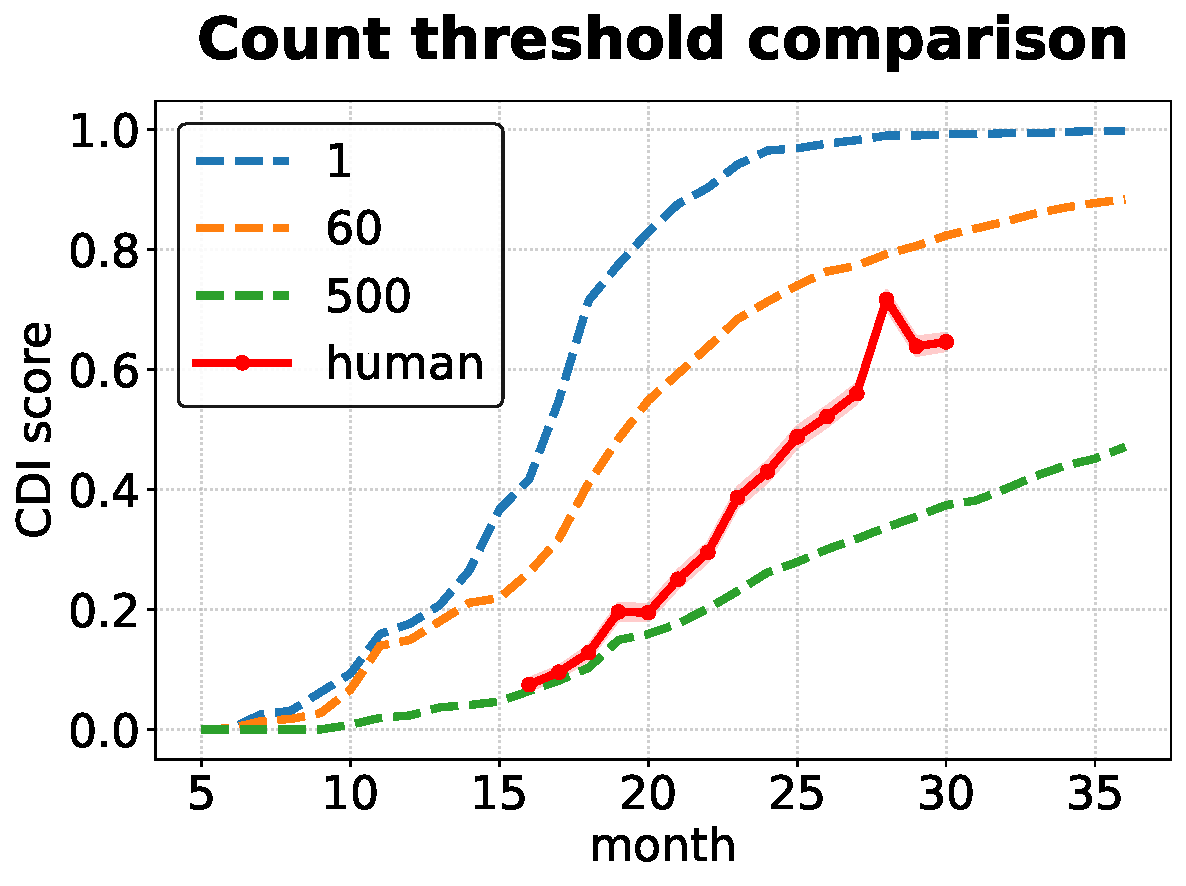
\includegraphics[width=0.5\textwidth]{fig/threshold.pdf}}
\caption{\textbf{Count-based calibration.} Child corpus vocabulary trajectories obtained with count thresholds of 1, 60, and 500, alongside the caregiver-report reference (red). The selected threshold of 60 is the calibration used in the main analysis. The curves illustrate the sensitivity of coverage and trajectory to the count criterion; their comparison does not by itself validate equivalence to caregiver reports.}
\label{fig:threshold}
\end{figure}


The frequency-matched evaluation list and the finite generation budget introduce distinct sampling choices. Figure~\ref{fig:distr} examines the second choice beyond the selected list by comparing training and generation word counts for an LSTM trained on 3.4M words, with generation volumes of 1, 10, and 100 times the reference amount. Larger output samples reduce the proportion of training words that are never generated, including in the lower-frequency range, but some rare words remain absent. The bottom panel therefore shows how observed absence changes as the sampling budget increases for a fixed trained model by the model. Absolute generated counts also rise mechanically with sample size, so movement in the scatter plot cannot alone be interpreted as improved learning or better-normalized word frequencies.


\begin{figure}[ht]
\centering
\subfloat{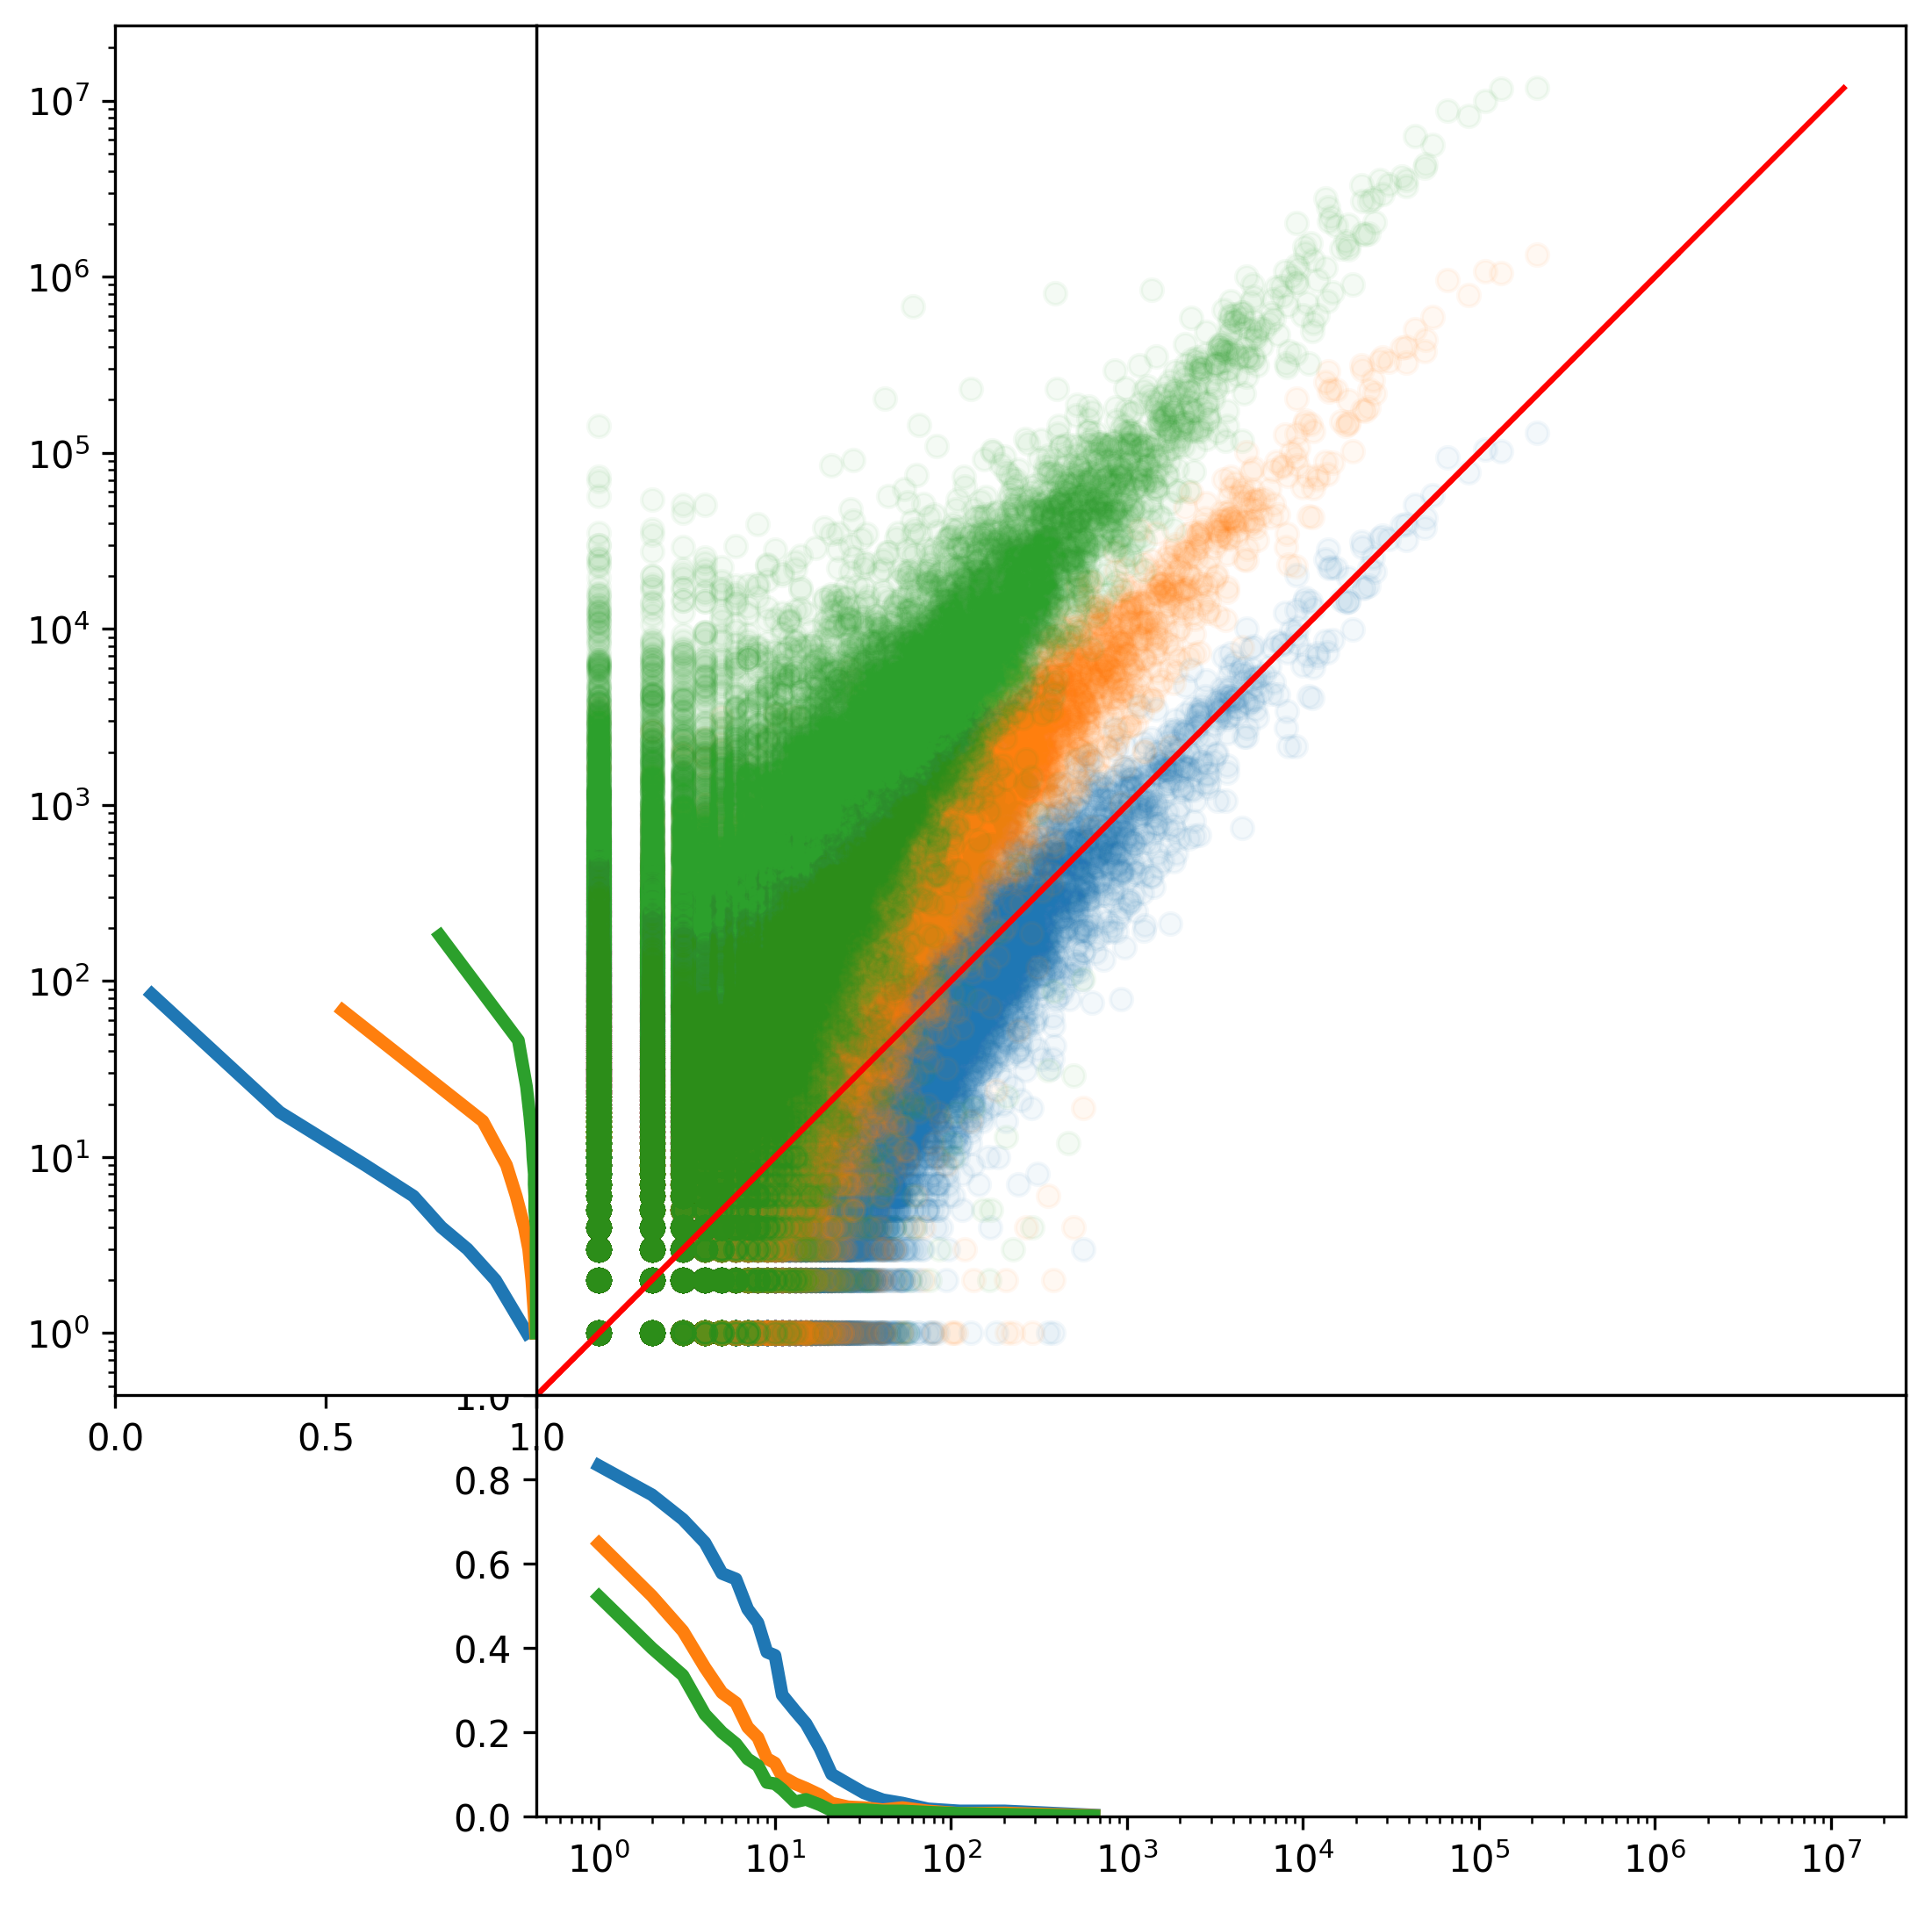
\includegraphics[width=0.3\textwidth]{fig/distr_LSTM_400.png}}
\hspace{1 pt}
\subfloat{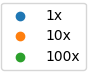
\includegraphics[width=0.1\textwidth]{fig/distr_cap.png}}
\caption{\textbf{Word count distribution(temperature = 1.0)}.Word frequency relationships between training and generation sets under different sampling conditions (1x, 10x, 100x generation volume). x-axis: word frequency in the training set; y-axis: word frequency in the generation set. The bottom panel shows the proportion of training word types absent from generated output as a function of their training count.}
\label{fig:distr}
\end{figure}


The exposure-scaling analysis in Figure~\ref{fig:hour} compares \meCDI{} trajectories under three estimated annual input budgets. Larger input budgets improve coverage in some conditions but do not reproduce the child reference trajectory within the tested protocol. This is evidence about the effect of the tested corpus-size manipulation, not identification of a unique learning mechanism responsible for the discrepancy.

\begin{figure}[ht]
\centering
\subfloat{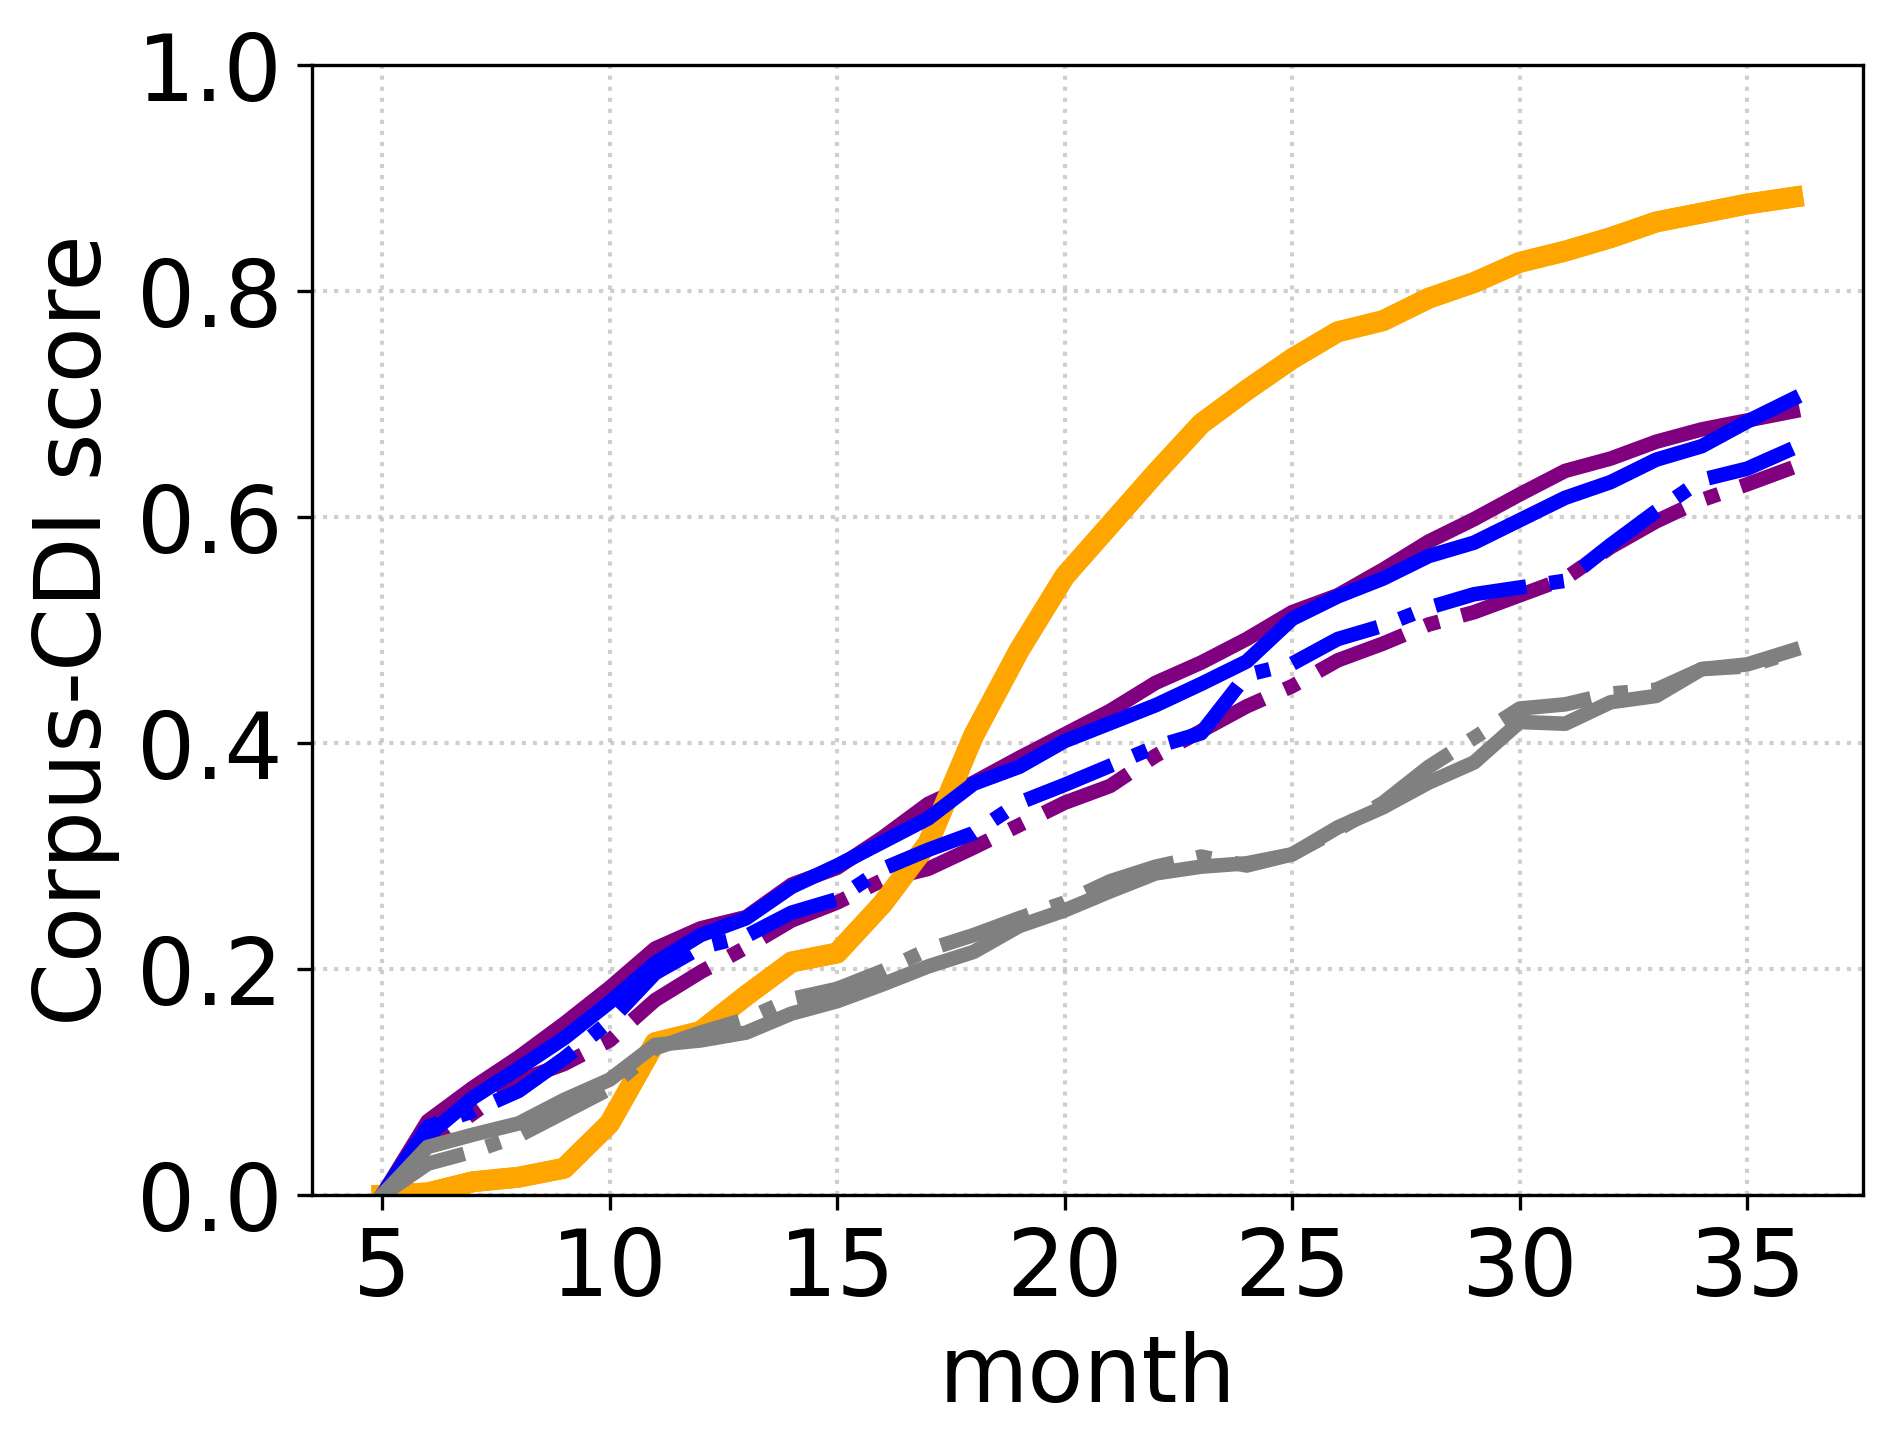
\includegraphics[width=0.35\textwidth]{fig/hour.png}}
\subfloat{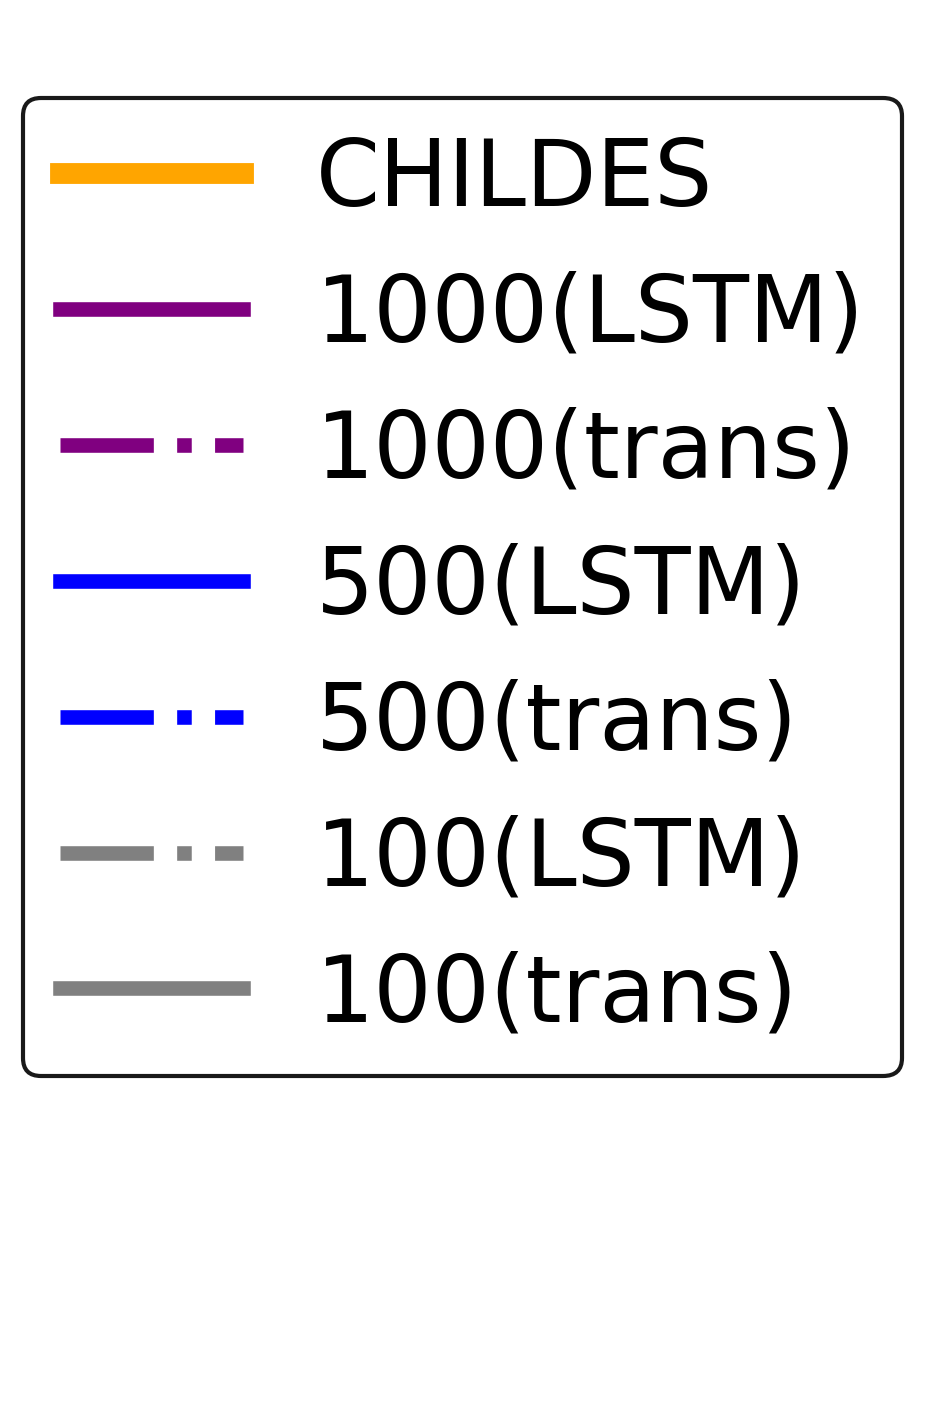
\includegraphics[width=0.1\textwidth]{fig/hour_legend.png}}
\caption{\textbf{Model vocabulary growth across estimated annual exposure levels.} Comparison of \meCDI{} trajectories for models trained on 100-, 500-, and 1000-hour exposure estimates, alongside CHILDES child production data. Models show roughly linear vocabulary growth that scales modestly with total exposure but remains far below the human developmental curve. }
\label{fig:hour}
\end{figure}
